%% Based on a TeXnicCenter-Template by Tino Weinkauf.
%%%%%%%%%%%%%%%%%%%%%%%%%%%%%%%%%%%%%%%%%%%%%%%%%%%%%%%%%%%%%

%%%%%%%%%%%%%%%%%%%%%%%%%%%%%%%%%%%%%%%%%%%%%%%%%%%%%%%%%%%%%
%% HEADER
%%%%%%%%%%%%%%%%%%%%%%%%%%%%%%%%%%%%%%%%%%%%%%%%%%%%%%%%%%%%%
\documentclass[a4paper,twoside,12pt]{report}
% Alternative Options:
%	Paper Size: a4paper / a5paper / b5paper / letterpaper / legalpaper / executivepaper
% Duplex: oneside / twoside
% Base Font Size: 10pt / 11pt / 12pt


%% Language %%%%%%%%%%%%%%%%%%%%%%%%%%%%%%%%%%%%%%%%%%%%%%%%%

\usepackage[T1]{fontenc}
\usepackage[left=2.5cm,right=2.5cm,top=2.5cm,bottom=2.5cm]{geometry}
\usepackage{lmodern} %Type1-font for non-english texts and characters
%\usepackage[latin1]{inputenc}
\usepackage[utf8]{inputenc}
\usepackage[french]{babel}
\usepackage{color}
\usepackage{natbib}
%% Packages for Graphics & Figures %%%%%%%%%%%%%%%%%%%%%%%%%%
\usepackage{graphicx} %%For loading graphic files
%\usepackage{subfig} %%Subfigures inside a figure
%\usepackage{pst-all} %%PSTricks - not useable with pdfLaTeX

%% Please note:
%% Images can be included using \includegraphics{Dateiname}
%% resp. using the dialog in the Insert menu.
%% 
%% The mode "LaTeX => PDF" allows the following formats:
%%   .jpg  .png  .pdf  .mps
%% 
%% The modes "LaTeX => DVI", "LaTeX => PS" und "LaTeX => PS => PDF"
%% allow the following formats:
%%   .eps  .ps  .bmp  .pict  .pntg


%% Math Packages %%%%%%%%%%%%%%%%%%%%%%%%%%%%%%%%%%%%%%%%%%%%
\usepackage{amsmath}
\usepackage{amsthm}
\usepackage{amsfonts}
\usepackage{textcomp}
\renewcommand{\thechapter}{\Roman{chapter}}
%\renewcommand{\thesection}{\Roman{section}}
\renewcommand{\thepage}{\roman{page}}
%\renewcommand{\baselinestretch}{1.2}
%% Line Spacing %%%%%%%%%%%%%%%%%%%%%%%%%%%%%%%%%%%%%%%%%%%%%
\usepackage{setspace}
%\singlespacing        %% 1-spacing (default)
\onehalfspacing       %% 1,5-spacing
%\doublespacing        %% 2-spacing
\usepackage{floatrow}
\floatsetup[table]{capposition=top}

\usepackage{titlesec}
\setcounter{secnumdepth}{4}
\setcounter{tocdepth}{2}
%% Other Packages %%%%%%%%%%%%%%%%%%%%%%%%%%%%%%%%%%%%%%%%%%%
%\usepackage{a4wide} %%Smaller margins = more text per page.
\usepackage{fancyhdr} %%Fancy headings
%\usepackage{longtable} %%For tables, that exceed one page
%d\'efinition des entêtes
\usepackage{url}
\pagestyle{fancy}
\usepackage [dvips]{epsfig}
\usepackage{hyperref}
 \usepackage[utf8]{inputenc} 
 \usepackage[T1]{fontenc} 
\usepackage{multicol}
\usepackage{setspace}
\usepackage{slashbox}
\setstretch{1,5}
\renewcommand{\familydefault}{ptm}
\selectfont
\addto\captionsfrench{\def\figurename{{Figure}}}
\addto\captionsfrench{\def\tablename{{Tableau}}}


%%%%%%%%%%%%%%%%%%%%%%%%%%%%%%%%%%%%%%%%%%%%%%%%%%%%%%%%%%%%%
%% DOCUMENT
%%%%%%%%%%%%%%%%%%%%%%%%%%%%%%%%%%%%%%%%%%%%%%%%%%%%%%%%%%%%%
\begin{document}
%\newfont{\mafonte}{cmr 12 at 13pt}
%\AtBeginDocument{\mafonte}

\normalsize{\fontsize{13}{13}\selectfont}
\fontsize{13}{13}\selectfont

\fancyhf{} % supprime les en-têtes et pieds pr\'ed\'efinis
%\fancyhead[LO,RE]{}% Left Even, Right Odd
%\fancyhead[L]{\bfseries\rightmark} % Left Odd
%\fancyhead[R]{\bfseries\leftmark} % Right Even
\fancyfoot[LE,LO]{}
\fancyfoot[RO,RE]{\thepage}
%\textbf{UNIVERSIT\'{E} DE MAROUA 2015 - 2016} } }
%\fancyfoot[LO,RE]{\tiny \textbf {Rédigé Mouafo } \textbf{\copyright} \textbf{ENS.MAROUA 2015}}
\renewcommand
{\footnoterule}{
\vspace*{0.5cm}
\hfill  \hfill 
}
\renewcommand{\headrulewidth}{1.pt}% filet en haut de page
\addtolength{\headheight}{4pt} % espace pour le filet
\renewcommand{\footrulewidth}{1.pt}% filet en bas de page
%\addtolength{\footheight}{10pt} % espace pour le filet en bas
\fancypagestyle{plain}{ % pages de tetes de chapitre
\fancyhead{} % supprime l'entete
%\fancyfoot{} %supprime le pied de page
\renewcommand{\headrulewidth}{0pt} % et le filet
%\renewcommand{\footrulewidth}{0pt}
}
\newcommand{\clearemptydoublepage}{%
\newpage{\pagestyle{plain}\cleardoublepage \renewcommand{\headrulewidth}{0pt}\addtolength{\headheight}{4pt}}
}
\lhead{\textsl{chapitre \thechapter}}
\rhead{\textsl{\leftmark }}

%\lfoot{\footnotesize{\textbf{Mémoire de MASTER II }}}
% Ceci permet d'avoir les noms de chapitre et de section
% en minuscules
\renewcommand{\chaptermark}[1]{\markboth{#1}{}}
\renewcommand{\sectionmark}[1]{\markright{\thesection\ #1}}
\renewcommand{\headsep}{20pt}


\chapter*{Dédicace}\addcontentsline{toc}{chapter}{Dédicace}
\vspace*{5cm}
\begin{flushright}
    \large\em\null\vskip1in 
     \`{A} maman LAKGUEM Suzanne \vfill
  \end{flushright}




%%%%%%%%%%%%%%%%
 
\chapter*{Remerciements}\addcontentsline{toc}{chapter}{Remerciements}

\hspace*{10pt}Un mémoire est un travail de recherche long et ardu. Malgré
que ce soit un travail en solitaire, il aurait été difficile d'occulter de l'appui de
nombreuses personnes d'un point de vue académique et moral, à qui je tiens à exprimer toute ma reconnaissance. Je tiens à exprimer mes remerciements et ma vive gratitude à : 
\begin{itemize}
		\item[\textbullet]	Pr. MOTAPON Ousmanou qui me fait l'honneur de présider ce jury de mémoire ;
		\item[\textbullet]  Dr. Tchangnwa  Nya Fridolin pour avoir accepté d'évaluer ce travail ;
		\item[\textbullet]  Prof. Dr.-Ing. habil. KOLYANG  qui a accepté d'être le rapporteur de ce mémoire, je le remercie tout particulièrement pour l'attention et le temps qu'il y a consacré ;
		\item[\textbullet]	Ma mère LAKGUEM Suzanne qui a cru en moi et m'a soutenu tout le long de mes études ;
		\item[\textbullet]  mes frères et sœurs, NIMPA Collins, LEBOU Ghislain, DASSE Odosine pour leurs soutiens financier et morale pendant toutes la durée de ma formation ;
		\item[\textbullet]	Mlle. LOBAWO Adeline Zoustel pour son amour, son soutien moral et ses encouragements ;
		\item[\textbullet]  la famille PASSO de Maroua pour m'avoir accueilli comme un fils. 
		\item[\textbullet]  tous les enseignants qui m'ont suivi tout au long de cette formation.
		\end{itemize}
	
	 Je remercie particulièrement ma famille pour le soutien qu'elle m'a apporté et la
motivation qu'elle a su me donner lorsque j'en avais le plus besoin.\\

 J'exprime  également  toute  ma  sympathie  et  ma  gratitude à mes collègues de stage, MOUAFO Joseph, ZANGUE Josue et les autres pour l'ambiance agréable qu'ils ont su créer.\\ 






%% Title Page %%%%%%%%%%%%%%%%%%%%%%%%%%%%%%%%%%%%%%%%%%%%%%%
%% ==> Write your text here or include other files.


%% The nice version:
%\input{titlepage} %%You need a file 'titlepage.tex' for this.
%% ==> TeXnicCenter supplies a possible titlepage file
%% ==> with its templates (File | New from Template...).


%% Inhaltsverzeichnis %%%%%%%%%%%%%%%%%%%%%%%%%%%%%%%%%%%%%%%
\tableofcontents %Table of contents

\chapter*{Liste des sigles et abréviations}\addcontentsline{toc}{chapter}{Liste des sigles et abréviations}

2DPCA : two Dimensional Principal Component Analysis

ACP : Analyse en Composantes Principales 

ADL : Analyse Discriminante Linéaire

ADN : acide désoxyribonucléique 

BD : Base de Données

BTS : Brevet de Technicien Supérieur

EBGM : Elastic Bunch Graph Matching

FRVT: Face Recognition Vendor Test

ID  : IDentifier

ISS : Institut Supérieur du Sahel

MIT : Massachussetts Institute of Technology

LBP : Local Binary Patterns

PC : Personal Computer

PCA : Principal Component Analysis

LTP : Local Trinary Patterns

SVM : Machine Vecteur Support


\chapter*{Résumé}\addcontentsline{toc}{chapter}{Résumé}

 La reconnaissance faciale est une technologie biométrique non intrusive et sans contact. Ces caractéristiques font d'elle un domaine de recherche aux publications abondantes. Bien que de nombreuses méthodes et techniques de reconnaissance de visage aient été proposées, elle reste encore un problème difficile, car les facteurs externes comme la variation d'illumination, la variation de pose et d'expressions faciales ne sont pas toujours traités de manière satisfaisante par la plupart des algorithmes. De nos jours les systèmes d'identification et de vérification biométrique constituent une alternative de taille à l'authentification traditionnelle.

Ce mémoire traite de l'identification automatique de visage sur une photo ou dans un flux vidéo. Deux méthodes de reconnaissance sont présentées : la méthode \textit{eigenface} qui utilise l'analyse en composantes principales et la méthode des "Local Binary Patterns". Ces deux algorithmes ont été testés sur les bases de données ORL et YALE et les résultats obtenus montrent que la technique LBP donne de meilleurs résultats.
 
\vspace{20pt}
\textbf{Mots clés :} Reconnaissance faciale, ACP, Eigenface, LBP

\chapter*{Abstract}\addcontentsline{toc}{chapter}{Abstract}
The applications of biometrics becoming more and more nowadays. Facial recognition is a non-intrusive and contactless biometric technology. These characteristics make it an area of ​​research with abundant publications. Although many methods and face recognition techniques have been proposed, it remains a difficult problem, because external factors such as illumination variation, variation of poses and facial expressions are not always treated satisfactory manner in most algorithms. Nowadays identification systems and biometric verification is a good alternative to traditional authentication.

This thesis treat of automatic face recognition on a photo or a video stream. Two recognition methods are presented: the Eigenface method using the principal components analysis and the Local Binary Patterns method (LBP). These two algorithms were tested on ORL and YALE database and the results show that LBP technical work best.

\vspace{20pt}

\textbf{Keywords} : face recognition, PCA,Eigenface, LBP



%% The List of Figures
\clearpage

\addcontentsline{toc}{chapter}{Liste des figures et illustrations}
\listoffigures

%% The List of Tables
\clearpage

\addcontentsline{toc}{chapter}{Liste des tableaux}
\listoftables


%\pagestyle{plain} %Now display headings: headings / fancy / ...




%%%%%%%%%%%%%%%%
 
\chapter*{INTRODUCTION}\addcontentsline{toc}{chapter}{INTRODUCTION}
\renewcommand{\thepage}{\arabic{page}}
\setcounter{page}{1}
%\thispagestyle{empty}
De nos jours, l'insécurité devient de plus en plus présente dans divers secteurs. Les secteurs les plus visés sont l'e-commerce, les opérations bancaires, militaires. Les moyens informatiques sont proposés pour lutter contre cette tendance parmi lesquels la méthode de contrôle d'accès. Le contrôle d'accès logique s'effectue en trois étapes : l'identification, l'authentification et l'autorisation. S'identifier, c'est se faire connaître du système tandis que s'authentifier c'est prouver son identité au système. Quant à l'autorisation, elle donne le droit d'effectuer une opération précise. Il existe deux manières d'authentifier un individu. La première méthode est basée sur \og ce que l'on connaît\fg{} de l'individu comme la connaissance d'un couple identifiant/mot de passe. La deuxième méthode est basée sur \og ce que l'on possède \fg{} par exemple la possession d'une pièce d'identité, d'un badge, d'une clé, etc. Ces deux méthodes peuvent être utilisées de manière complémentaire dans le but d'accroître la sécurité mais présente chacune des faiblesses. Par exemple un mot de passe peut être oublié, volé ou deviné par autrui. De même une pièce d'identité (ou clé) peut être perdue, volée par une personne mal intentionnée.\\

\hspace*{10pt}La biométrie est une technique globale visant à établir l'identité d'une personne en mesurant une de ses caractéristiques physiques. Roethenbaugh \citep{Roe12} définit la biométrie de la façon suivante : \og \textit{La  biométrie  s'applique à des particularités ou des caractères humains uniques en leur genre et mesurables, permettant de reconnaître ou de vérifier automatiquement l'identité}\fg{}. Les caractéristiques biométriques constituent ainsi une solution alternative aux deux méthodes d'authentification évoquées précédemment. Elles présentent l'avantage d'être uniques et présentes chez toutes les personnes à identifier.\\

\hspace*{10pt}Il existe différents types de technologies biométriques à savoir la reconnaissance faciale, la reconnaissance d'empreintes digitales, l'identification de la géométrie des doigts et de la main, l'identification de l'iris, l'identification de la voix, l'identification de la signature, etc.\\

\hspace*{10pt}La reconnaissance faciale est une aptitude qui relie l'apparence d'une personne à son identité. La capacité pour l'identification de visage est très importante pendant notre vie sociale. Chacun de nous identifie tout le long de la journée différents visages. A la rencontre d'une nouvelle personne, notre cerveau recherche dans notre mémoire si cette personne est répertoriée ou non. La reconnaissance faciale permet ainsi de construire une relation à long terme où les individus finissent par se connaître. \\

\thispagestyle{empty}

\hspace*{10pt}Grâce à la puissance croissante de l'informatique et aux prix décroissants des ordinateurs, des applications informatiques sont appliquées populairement dans notre vie quotidienne. Dans le domaine de la vision par ordinateur, la reconnaissance de visage a attiré beaucoup l'attention des chercheurs. Malgré que plusieurs idées intéressantes et utiles soient déjà proposées, ce problème n'est pas souvent traité complètement. Et il est encore un problème ouvert qui demande plus d'étude profonde. En fait, ce problème n'est pas simplifié.

La reconnaissance faciale a de nombreux champs d'applications : télésurveillance, vérification d'identité pour le déverrouillage d'ordinateur ou la traque de suspects à travers les enregistrements vidéo, reconnaissance des expressions faciales, etc. 

Nous avons choisi d'articuler notre étude autour de cinq chapitres principaux. Le chapitre 1 présente le contexte de notre travail ainsi que la problématique sur laquelle il se base. Le deuxième chapitre est consacré aux généralités sur les systèmes biométriques, il décrit quelques systèmes biométriques ainsi que leur principe de fonctionnement. Ensuite la place de la reconnaissance faciale parmi les autres techniques biométriques est analysée. Enfin nous présentons les difficultés rencontrées dans les systèmes de reconnaissance faciale. Dans le chapitre 3, nous présentons un état de l'art sur les techniques et méthodes de détection et de reconnaissance de visages. Dans le chapitre 4, nous expliquons comment nous avons développé un système de reconnaissance faciale utilisant les algorithmes eigenface et LBP. Enfin dans le cinquième et dernier chapitre, nous présentons les résultats et tests de performance que nous analyserons.





\nocite{MAL}






%%%%%%%%%%%%%%%%
 
\chapter{CONTEXTE ET PROBLÉMATIQUE}

\hspace*{10pt} Dans ce chapitre, nous présentons d'abord brièvement la structure dans laquelle
nous avons effectué notre stage de fin d'étude, le contexte, puis la problématique sur laquelle notre travail est basé. Ensuite viendront les objectifs fixés ainsi que la méthodologie adoptée pour parvenir à bout de ces objectifs. 
\section{Présentation de la structure de stage}
Notre stage de fin de formation s'est déroulé du 03 mars au 10 juillet 2016 au laboratoire informatique de l'Institut Supérieur de Sahel (ISS) de l'Université de Maroua. L'ISS est l'une des grandes écoles de l'Université de Maroua. Ouvert en 2008, sa principale mission est de former de jeunes étudiants dans les domaines de :
\begin{itemize}
	\item  [\textbullet] Agriculture, Élevage et Produits Dérivés (AGEPD) ;
	\item  [\textbullet] Beaux-arts et science du patrimoine (BEARSPA) ;
	\item  [\textbullet] Climatologie, Hydrologie et Pédologie 
	\item  [\textbullet] Énergies renouvelables (ENREN) ;
	\item  [\textbullet] Hydraulique et Maîtrise des eaux (HYMAE) ;
	\item  [\textbullet] Informatique et Télécommunications (INFOTEL) ;
	\item  [\textbullet] Génie du Textile et Cuir (GTC) ;
	\item  [\textbullet] Sciences Environnementales (SCIENV) ;
	\item  [\textbullet] Sciences Sociales pour le Développement (SCISOD) ;
	\item  [\textbullet] Traitement des Matériaux, Architecture et Habitat (TRAMARH).
\end{itemize}
Dans chaque département, les formations sont offertes en deux cycles : le cycle ingénieur des travaux dont la durée est de trois ans et le cycle ingénieur de conception pour une durée de cinq ans. A l'exception du département de Climatologie qui offre en plus un cycle BTS.

Le laboratoire informatique de l'ISS et le département d'INFOTEL partagent le même bâtiment au campus de pitoré (IRAD) et sont tous dirigés par Dr. VIDEME BOSSOU Olivier. 

\section{Contexte}

De nos jours, la fraude ne cesse d'augmenter dans la société. Certains
utilisateurs, (imposteurs) sont capables de falsifier leur identité avec une
facilité remarquable. Ceci est dû au fait que les systèmes d'authentification les
plus utilisés sur le marché sont basés sur la solution conventionnelle: \og login and
password\fg{} ou accès avec mot de passe, souvent associée à une carte ID
contenant l'information sur d'identité de son possesseur. Cependant, les
utilisateurs ne sont pas tout à fait satisfaits de ces cartes ID pour les raisons
suivantes:
\begin{itemize}
	\item les cartes ID basées sur les mots de passe ne sont pas fiables,
	\item les cartes ID peuvent être perdues, oubliées ou mal placées,
	\item le mot de passe risque d'être oublié ou compromis.
\end{itemize}
Les utilisateurs ne se sentent pas suffisamment bien sécurisés en effectuant des transactions faisant appel à de telles techniques d'authentification.  

Une étude \footnote{Cette étude intitulée : « Businesses Should Begin Preparing for the Death of the Password » a été réalisée par OnePoll.com pour Gigya, en février 2016, auprès de 2 000 adultes américains et 2 000 adultes britanniques entre 18 et 69 ans ayant accès à Internet et étant titulaires de comptes en ligne.} menée auprès de 4 000 consommateurs aux Etats-Unis et au Royaume-Uni \cite{BIOM}a montré que 52\% des consommateurs  choisiraient si on leur proposait  une autre option que celle de la traditionnelle \og login/mot de passe\fg{} pour s'inscrire sur un site web ou sur une application. Selon \cite{BIOM}, 25\% ont été victime d'une compromission de leur compte au cours des 12 derniers mois. Ce taux monte à 35\% pour la génération Y \footnote{La génération Y regroupe des personnes nées approximativement entre le début des années 1980 et le milieu des années 1990.}, car souvent moins rigoureux dans la détermination de leur mot de passe. Certaines entreprises complexifient leur politique de génération de mot de passe, mais cela alourdi les procédure d'inscription et décourage certains utilisateurs.

Les entreprises doivent donc moderniser leurs méthodes d'authentification sous peine d'en subir les conséquences. La plupart se tournent vers la biométrie. 
\section{Problématique}

Face aux différents problèmes que posent les méthodes traditionnelles, on se demande comment construire un système d'authentification physique en temps réel et qui donne le plus de confort aux utilisateurs tout en garantissant un accès hautement sécurisé? 

\section{Objectifs}
Différents types de systèmes sont utilisés pour l'identification/authentification en temps réel. Les  plus  populaires  sont  basés  sur  le  visage, l'empreinte digital et l'iris. Notre objectif est de proposer un système biométrique basé sur la reconnaissance faciale respectant des contraintes  temps  réels.

\section{Méthodologie}
Pour résoudre ce problème, nous allons dans un premier temps répertorier les différents techniques et algorithmes de reconnaissance faciale, ensuite étudier leur performances et enfin implémenter le système qui convient le mieux (c'est-à-dire celui qui respecte les conditions temps réel et qui admet un taux acceptable de reconnaissance), puis procéder à des tests de validation. 
 




%%%%%%%%%%%%%%%%
 
\chapter{GÉNÉRALITÉS SUR LA RECONNAISSANCE FACIALE}

\section{Introduction}
La biométrie ou plus précisément la reconnaissance biométrique est \og \textit{l'exploitation automatisée ou semi-automatisée de caractéristiques physiologiques ou comportementales pour déterminer ou vérifier l'identité}\fg{}\citep{bio}.
De nos jours les systèmes biométriques sont de plus en plus utilisés dans la société. Par exemple facebook utilise la reconnaissance faciale pour identifier les individus sur une image nouvellement publiée. La détection de visages est utilisé dans les récents appareils photos numériques pour mettre au point les prises. Le dispositif de Schiphol Privium à l'aéroport d'Amsterdam, utilise un capteur  de  l'iris  pour  accélérer  la  procédure  de  contrôle  des  passeports  et  des  visas \citep{cnn}.

\section{Les systèmes biométriques}
 Les systèmes biométriques sont très diverses selon la caractéristique physique prise en compte : 
\begin{itemize}
	\item les empreintes digitales
	\item le visage
	\item l'ADN
	\item la géométrie de la main
	\item l'iris
	\item la rétine
	\item la voix
	\item la dynamique des signatures
	\item ...
\end{itemize}

Les statistiques des systèmes biométriques sur le marché sont résumés dans le diagramme ci-après.

\begin{figure}[htbp]
	\centering
		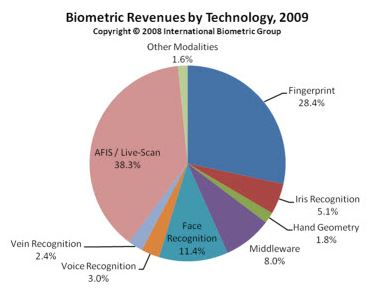
\includegraphics{market.JPG}
	\caption{marché des différentes technologies biométriques}
	\label{fig:market}
\end{figure}

\subsection{Caractéristique biométrique}
 Pratiquement, n'importe quelle caractéristique physiologique ou comportementale peut être considérée comme une caractéristique biométrique, mais elle doit répondre aux critères ci-dessous \citep{Lal} : 
\begin{itemize}
	\item [\textbullet] \textbf{universalité} : la caractéristique doit être présente chez toute personne.
	\item [\textbullet] \textbf{unicité} : pour identifier ou authentifier une personne dans une population, il est nécessaire que la caractéristique biométrique utilisée soit unique à cette personne.
	\item [\textbullet] \textbf{permanence} : la caractéristique doit être suffisamment immuable pendant une période donnée. 
	\item [\textbullet] \textbf{perceptibilité} : la caractéristique doit pouvoir être mesurée quantitativement.  
\end{itemize}
Pour utiliser un système biométrique, plusieurs facteurs doivent être prises en compte au milieu desquels :
 
 \begin{itemize}
	 \item [\textbullet] \textbf{performance} : il s'agit de la fiabilité et de la rapidité de reconnaissance du système, des ressources requises et de l'influence de l'environnement sur le fonctionnement du système.
	\item [\textbullet] \textbf{acceptabilité} : ce facteur traduit la manière dont les gens sont disposés à accepter l'utilisation du système. 
	\item [\textbullet] \textbf{facilité de contournement} : facilité avec laquelle la sécurité du système peut être déjouée.
 \end{itemize}


\subsection{Modes de fonctionnement d'un système biométrique}

Un système biométrique peut fonctionner en trois modes selon le contexte d'utilisation :
\begin{itemize}
	\item [\textbullet] le mode d'\textbf{enrôlement} : c'est une phase d'apprentissage dont le principal but est de recueillir les informations biométriques des individus à identifier. Ces informations sont saisies par un capteur biométrique, puis stockées dans une base de données.
	
	\item [\textbullet] le mode de \textbf{vérification} ou d'\textbf{authentification} : dans ce mode, le système répond à la question \og \textit{Suis-je réellement la personne que je suis en train de proclamer ?}\fg{}\citep{Sou12}. Le système compare les données biométriques saisies avec le modèle biométrique de personne à authentifier (préalablement stockée dans la base de données). C'est une comparaison de type "1 à 1".
	
	\item [\textbullet] le mode d'\textbf{identification} : dans ce mode, le système répond à la question \og \textit{Qui suis-je ?}\fg{}. Une identité est associée à une personne en l'appariant avec l'un des modèles de la base de données. C'est une comparaison de type "1 à N".
\end{itemize}
 Ces différents modes sont résumés dans la figure ci-dessous.
\begin{figure}[htbp]
	\centering
		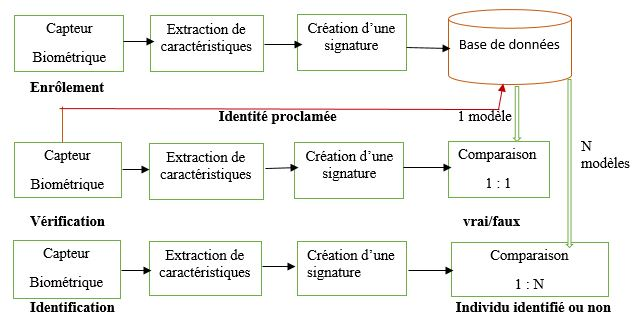
\includegraphics{mode.JPG}
	\caption[modes de fonctionnement d'un système biométrique]{modes de fonctionnement d'un système biométrique (source \cite{Sou12}}
	\label{fig:mode}
\end{figure}

La figure \ref{fig:mode} représente les différents modules qui composent un système biométrique. Leur fonctionnement peut être résumé comme suit :
\begin{itemize}
	\item module capteur biométrique : système d'acquisition équipé d'un terminal de capture biométrique ou capteur biométrique utilisé pour acquérir une caractéristique spécifique de l'utilisateur, par exemple: une caméra ou un microphone dans le cas de la voix.
	\item module d'extraction de données : ayant une image ou une voix en entrée, une étape de segmentation permet d'extraire la caractéristique dont le processus d'authentification/identification a besoin. Par exemple : extraire le visage du fond d'une image dans le cas de l'identification de visage.
	\item module création d'une signature : crée un modèle numérique (ou signature) afin de représenter la 
donnée biométrique acquise. Cette signature est ensuite stockée dans une base de données.
  \item module  comparaison : compare les caractéristiques biométriques d'une personne soumise à contrôle avec les signatures mémorisées.
	\item module base de données : stocke les modèles biométriques des utilisateurs enrôlés.
\end{itemize}



\section{La reconnaissance faciale}
La reconnaissance de visage connaît un grand intérêt auprès de la communauté scientifique. C'est un domaine de recherche aux publications foisonnantes en raison de ses nombreuses applications. Parmi celles-ci les applications de surveillance, de contrôle d'accès dans les lieux publics (aéroports, banques et administrations) et bien d'autres.
Si la reconnaissance de visage apparaît comme un acte naturel et facile chez l'homme, il n'en est pas de même pour un ordinateur. Pour lui, c'est une suite de traitements complexes reposant sur des algorithmes complexes. La reconnaissance automatique de visage s'effectue en trois étapes : la \textbf{détection de visage,} l'\textbf{extraction des caractéristiques du visage} et l'\textbf{identification} et/ou \textbf{vérification}. 


\begin{figure}[htbp]
	\centering
		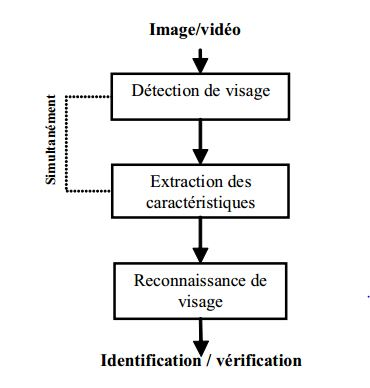
\includegraphics[height=200pt]{etape.JPG}
	\caption{étapes de la reconnaissance faciale}
	\label{fig:etape}
\end{figure}

 
	\subsection{Quelques logiciels gratuits et produits commerciaux}
Le lecteur d'image Picasa de Google intègre une implémentation de la reconnaissance faciale. Il peut associer des visages aux personnes. De même IPHOTO d'Apple utilise un système capable d'étiqueter les visages reconnus sur une photos.  Les systèmes de reconnaissance des visages sont déployés  dans le  transport aérien, le système \og Smart  Gate \fg{} par exemple a été mis en  œuvre  afin d'effectuer  une vérification automatique de l'identité pour l'équipage d'Aéronef traversant la frontière de  l'Australie. Ce dernier  effectue  une  comparaison  entre  le  visage  d'une  personne  à  sa  photographie  de passeport.
Plusieurs entreprises ont orienté leurs activités vers la reconnaissance faciale à l'instar de \og Widget\fg{} par son système \og  Snappy Face\fg{} qui permet d'identifier le visage du propriétaire de l'ordinateur pour sécuriser son accès grâce à une webcam. 

Nous avons ci-dessous quelques produits commerciaux qui font des tâches similaires \citep{Gur}.
\begin{table}[htbp]
	\centering
		\begin{tabular}{|l|l|}
		\hline	Produit commercial & Site Internet \\ 
		\hline	FaceIt from Visionics & http://www.FaceIt.com\\
		\hline	Visage Technology  &http://www.viisage.com\\
		\hline	FaceVACS from Plettac & http://www.plettac-electronics.com\\
		\hline	SpotIt for face composite & http://spotit.itc.it/SpotIt.html\\
		\hline	ImageWare Sofware & http://www.iwsinc.com/ \\
		\hline	Cognitec Systems & http://www.cognitec-systems.de \\
		\hline	Visionsphere Technologies &  http://www.visionspheretech.com/menu.htm\\
		\hline	Biometric Systems & http://www.biometrica.com/ 	\\
		\hline
		\end{tabular}
	\caption{produits commerciaux de reconnaissance faciale}
	\label{tab:produitsCommerciauxDeReconnaissanceFaciale}
\end{table}
\subsection{Pourquoi la reconnaissance de visage?}
 Les caractéristiques  biométriques les plus communément utilisés sont les empreintes digitales. Le premier système d'authentification utilisant les empreintes digitales	fut commercialisé au début des années 80. Une autre caractéristique biométrique beaucoup plus fiable est l'iris car il garde la même texture au cours de la vie. Depuis quelques années, la reconnaissance de visage prend de plus en plus de l'ampleur. Ceci est dû au besoin du monde actuel, mais aussi de ses avantages parmi lesquels on peut citer : 
\begin{itemize}
	\item \textbf{les systèmes de capture} : caméras et appareils photo numériques sont hautement disponibles et à coûts raisonnables, sont faciles à installer et sont acceptables dans les lieux publics.
	\item la\textbf{ passivité} des systèmes à reconnaissance de visages : aucune coopération de la part du sujet à reconnaître n'est nécessaire. Le sujet n'a qu'à se promener devant une caméra pour être identifié. La reconnaissance de visage apparaît donc comme une technique appropriée pour l'identification des individus avec qui on ne peut coopérer, par exemple lors d'une poursuite de suspects.
\end{itemize}
La reconnaissance de visages n'est pas la plus fiable comparée à d'autres systèmes biométriques \cite{Sou12} mais donne de bons résultats lorsque de bonnes approches sont utilisées.


\subsection{Détection de visage}
Le visage humain est la source de diverses informations. Il constitue un vecteur visuel principal à l'identité d'un individu.
La détection de visage est le point d'entrée de tout système de reconnaissance faciale, car pour reconnaître une personne sur une vidéo ou sur une photo, il faut d'abord localiser son visage. Plusieurs travaux de recherches ont été effectués dans le domaine de la détection de visage et diverses méthodes ont été développées (voir section \ref{detection}). L'efficacité d'un système de reconnaissance faciale dépend donc de la technique de détection utilisée.


\subsection{Extraction de caractéristiques du visage}
L'étape d'extraction de caractéristiques constitue le cœur d'un système de reconnaissance, elle consiste à obtenir une représentation plus simple de l'image contenant seulement des informations utiles, discriminantes et non redondantes. Le but est de permettre une meilleure exploitation des données. L'extraction de paramètres peut concerner une région entière du visage (méthode globale) ou un des points particuliers de ses différentes régions caractéristiques comme le nez, la bouche, les coins des yeux\ldots Dans ce second cas, la méthode d'extraction est dite globale. Toutefois, ces deux catégories de méthodes peuvent être utilisées de manière complémentaire (méthodes hybrides).


\subsection{Reconnaissance de visage}
C'est la dernière étape du processus de reconnaissance faciale. Pendant cette phase, les caractéristiques obtenues à l'étape précédente sont utilisées pour créer une signature propre à chaque visage. Cette dernière est ensuite stockée dans une base de données. \`{A} chaque signature de la base correspond donc le visage d'un individu. Ainsi reconnaître un visage consiste donc à extraire sa signature et la mettre en correspondance avec la signature la plus proche dans la base de données. La reconnaissance peut se faire en mode vérification ou identification.

\section{Difficultés de la reconnaissance faciale}
 Si pour le cerveau humain, le processus de reconnaissance de visage est une tâche visuelle de haut niveau, il n'en est pas de même pour un système automatique de reconnaissance faciale. Construire un système capable d'identifier et de reconnaître un visage dans des conditions d'acquisition très variables est un sérieux défi à relever. On distingue deux types de variations associées aux images de visages : inter et intra sujet. La variation inter-sujet n'est rien d'autre que la ressemblance physique entre individu. Quant à la variation intra-sujet, elle est plus vaste et concerne plusieurs facteurs parmi lesquels la variation de l'éclairage, le changement de la position du visage lors de l'acquisition de l'image, etc. Nous analysons ci-dessous les facteurs les plus influents.

\subsection{Changement d'illumination }

La variation d'éclairage (distribution de la source de lumière, son intensité, son spectre) est un facteur très influent dans la tâche de reconnaissance de visage. Elle change l'apparence du visage, rendant ainsi très difficile sa reconnaissance. Adini et al. ont montré de manière expérimentale dans \citep{Adi} avec une base de données de 25 individus que le changement d'un visage dû à l'illumination peut s'avérer plus critique que la différence physique entre individus. 
\begin{figure}[htbp]
	\centering
		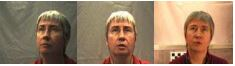
\includegraphics[height=100pt, width=300pt]{illumination.JPG}
	\caption[exemple de variation d'illumination]{exemple de variation d'illumination (source : \cite{Sou12})}
	\label{fig:illumination}
\end{figure}
Ce type de difficulté peut être surmontée par un prétraitement de normalisation et de compensation de l'illumination.
\subsection{Expressions faciales}
L'expression  faciale  est  une  mimique\footnote{jeu de physionomie}  faciale  chargée  de  sens.  Le  sens  peut  être l'expression  d'une  émotion,  un  indice  sémantique  ou une  intonation  dans  la  Langue  des 
Signes. Les  expressions faciales (voir \ref{fig:expression}) entraînent une déformation du visage qui est localisée principalement sur sa partie inférieure. La partie haute reste quasi-invariable et est suffisante pour effectuer une identification. Toutefois, l'expression faciale entraîne une diminution du taux de reconnaissance.
\begin{figure}[htbp]
	\centering
		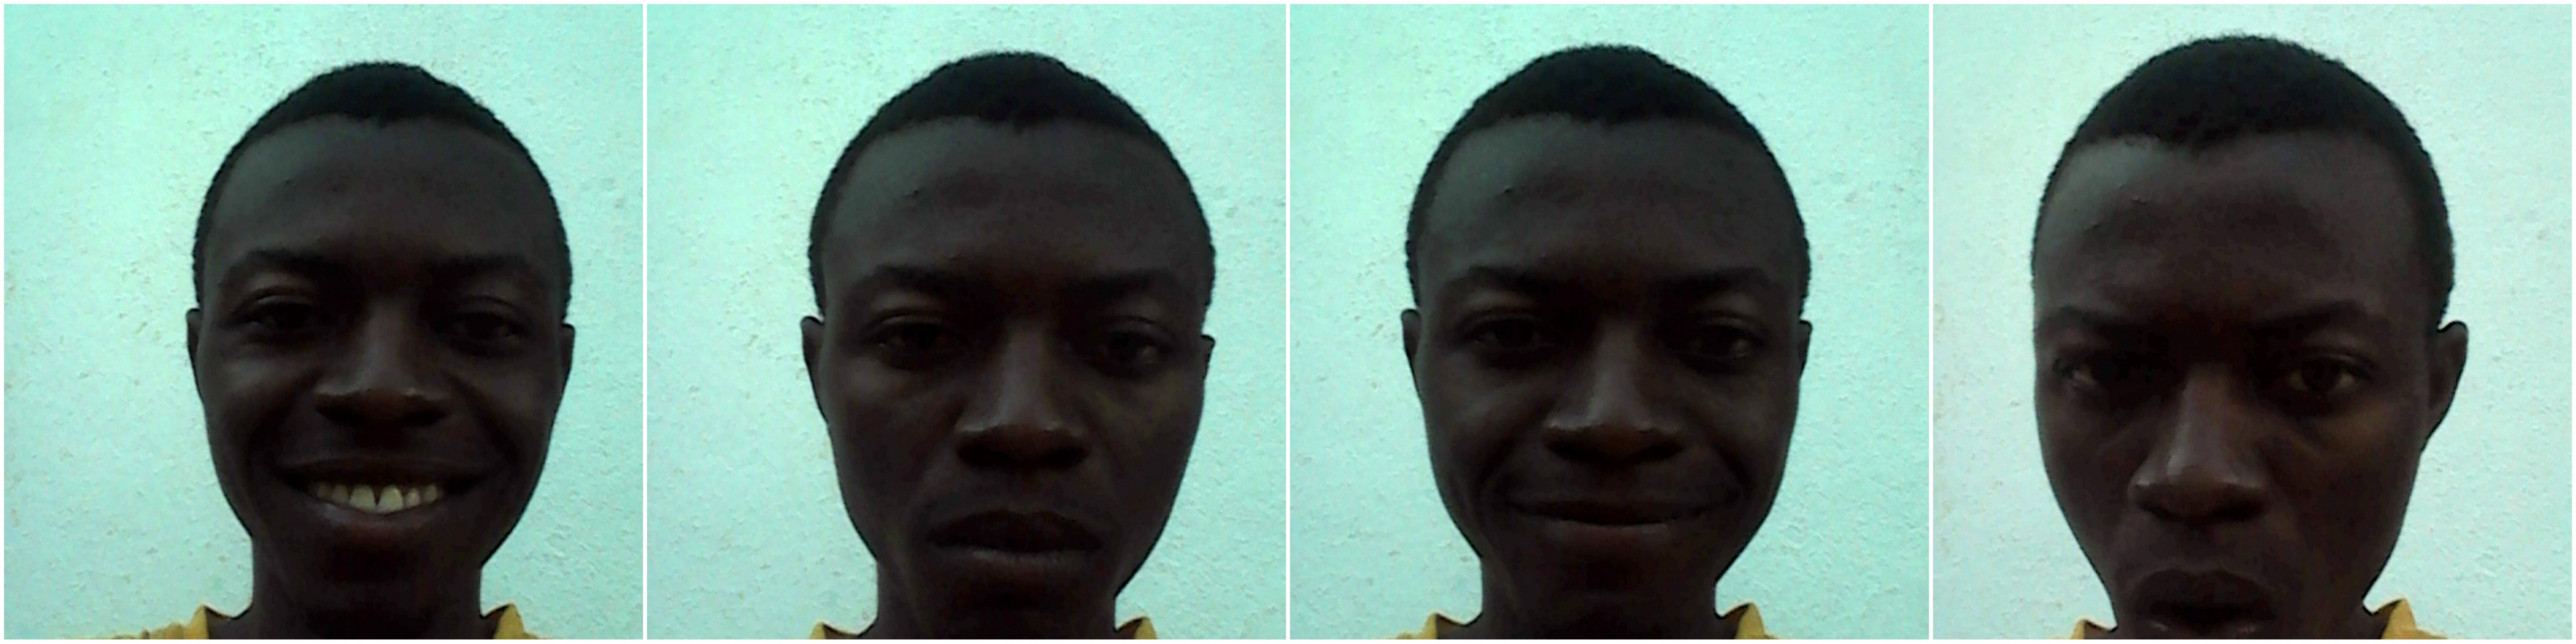
\includegraphics[height=100pt, width=400pt]{expression.jpg}
	\caption{exemple d'expressions faciales}
	\label{fig:expression}
\end{figure}
 
\subsection{Variation de pose}
La variation de pose (figure \ref{fig:pose}) est considérée comme l'un des problèmes majeurs de la reconnaissance de visage. Blackburn et al. dans \citep{Bla01} ont montré cette difficulté en effectuant des tests sur les bases de données FERET\footnote{http://www.itl.nist.gov/iad/humanid/feret/ visité le 24/04/2016} et FRVT\footnote{http://www.frvt.org visité le 24/04/2016}. Selon Blackburn et al., le visage peut être normalisé en détectant au moins  deux  traits  faciaux  (passant  par  les  yeux) quand il est de profil dans le plan image (orientation < 30\degres).  Cependant,  lorsque  la  rotation  est supérieure à 30\degres, la normalisation géométrique n'est plus possible.
\begin{figure}[htbp]
	\centering
		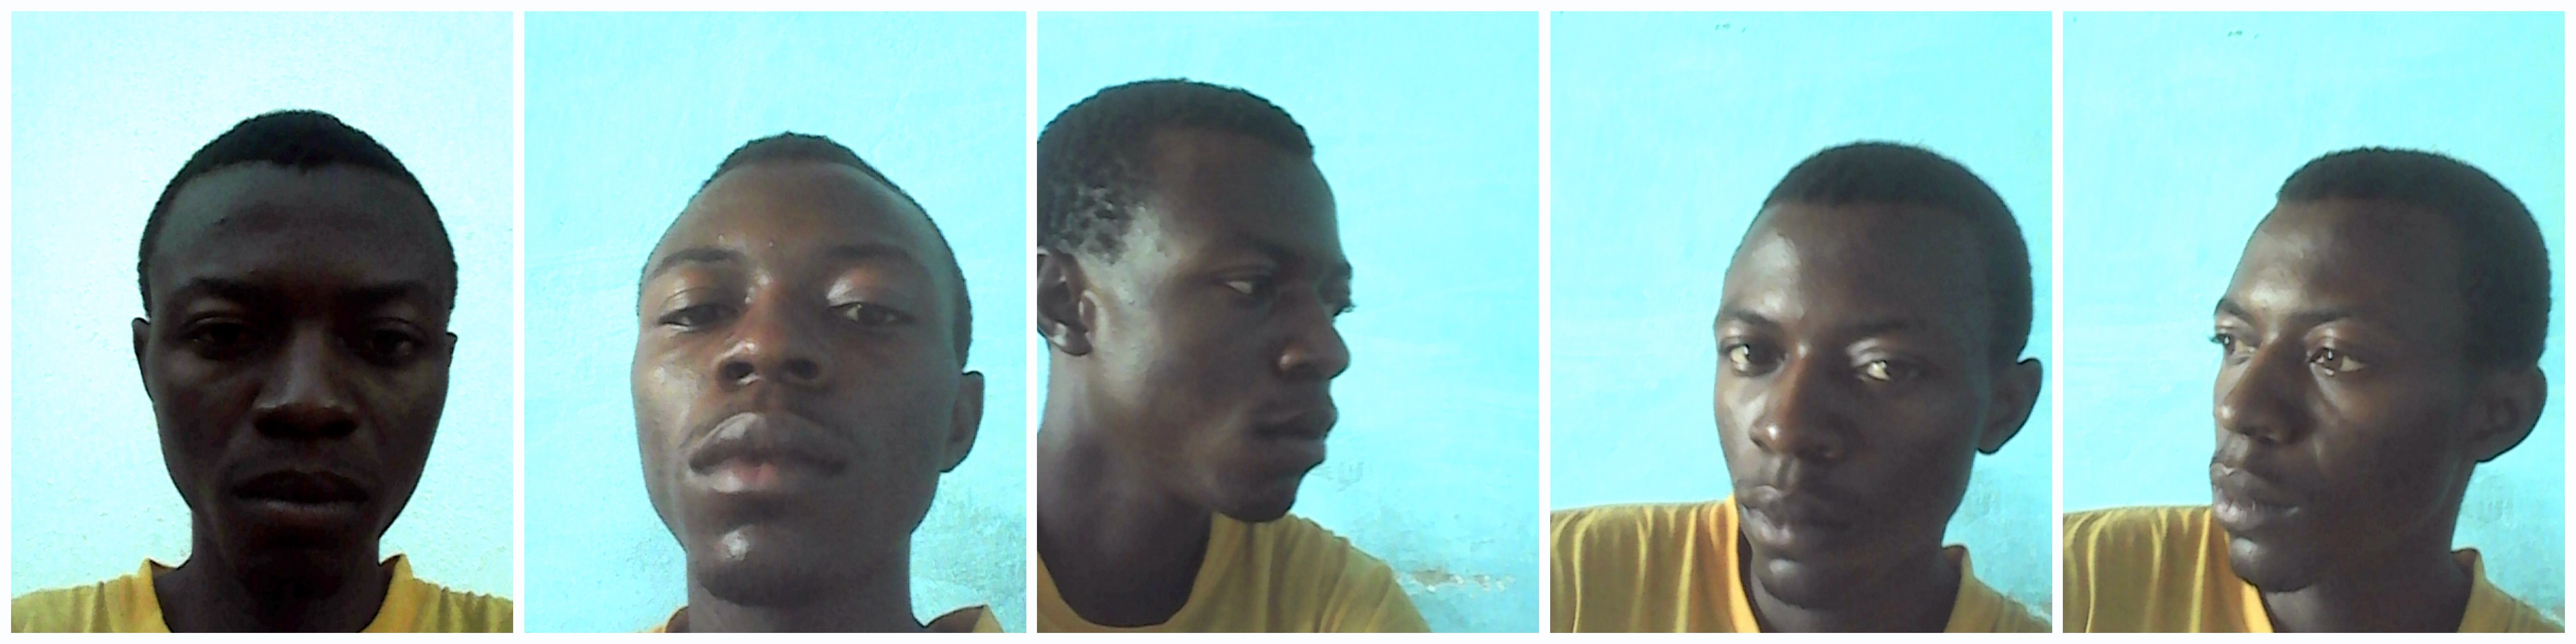
\includegraphics[height=100pt, width=400pt]{pose.jpg}
	\caption{exemple de variation de pose}
	\label{fig:pose}
\end{figure}
 
\subsection{Présence ou absence des composants structurales}
Il s'agit ici des éléments comme la barbe, la moustache, les lunettes, etc. Leur présence sur un visage peut modifier énormément les caractéristiques faciales telles que la forme, la taille ou la couleur du visage entraînant une défaillance ainsi du système de reconnaissance. 

\subsection{Occultations partielles}

Le visage peut être partiellement masqué par des objets dans la scène, ou par le port d'accessoires comme cache-nez, lunettes de soleil, écharpe\ldots Gross et al. dans \cite{Gro} ont étudié l'effet du port de lunettes 
de soleil, et du cache-nez occultant la partie inférieure du visage sur la reconnaissance faciale. Il ressort de cette étude que les performances des algorithmes restent faibles en cas d'occultations partielles de visage.

\subsection{Vrais jumeaux}
Même pour l'homme, reconnaître les vrais jumeaux n'est pas chose facile surtout lorsque l'on est moins familier avec eux. Il est peu probable que la vérification automatique de visage, ne pourra jamais détecter les 
différences très subtiles qui existent entre les vrais jumeaux.


\section{Conclusion}
Nous avons présenté dans ce chapitre les différents systèmes biométriques utilisés pour l'identification/authentification de personnes. L'accent a été mis sur la place qu'occupe la reconnaissance faciale au milieu des techniques biométriques.  Enfin, nous avons mis en évidence les différentes difficultés inhérentes à la reconnaissance automatique de visages. Dans le chapitre suivant, un état de l'art de la reconnaissance faciale sera présenté.
\hspace*{10pt}

\nocite{}

\chapter{ÉTAT DE L'ART DE LA RECONNAISSANCE FACIALE }

\section{Introduction}
La mise en œuvre d'un système automatique et fiable de reconnaissance faciale est un verrou technologique qui n'est toujours pas résolu. Plusieurs études ont été menées à  ce sujet. Je présente dans ce chapitre un état de l'art sur les techniques les plus significatives de détection, puis de reconnaissance de visage. Enfin je ferai une synthèse des méthodes et techniques étudiées.

\section{Techniques de détection de visage}
\label{detection}
La détection de visage pose le problème de la localisation des visages présents dans une image d'entrée. Depuis quelques années, les recherches dans le domaine de la détection des formes, des objets ainsi que celle des visages s'intensifient et ont donné naissance à plusieurs techniques de détection de visages. Ces différentes techniques sont classifiées par Yang et al. dans \citep{Yan01} de la manière suivante :
\begin{itemize}
	\item \textbf{Méthodes basées sur les caractéristiques invariables} (feature invariant approaches) : \\
	Ces approches utilisent les éléments invariants aux variations d'illumination, d'orientation ou d'expression tels que la texture ou
la signature de couleur de la peau pour la détection.


	\item \textbf{Méthodes basées sur la connaissance} :
	
	Comme leur classe indique, les méthodes basées sur la connaissance (knowledge-based methods en anglais) utilisent les connaissances sur les différents éléments qui constituent le visage, ainsi que les relations existants entre eux. La classification "visage | non visage" est effectuée en mesurant les positions relatives de différents éléments clés tels que la bouche, le nez et les yeux. L'inconvénient de ces méthodes est qu'elles n'arrivent pas à détecter un visage sur un arrière plan complexe.
	
	
	\item \textbf{Méthodes basées sur la correspondance avec les modèles} ("template matching methods") :\\ 
	Pour ces méthodes, des modèles caractéristiques (templates) d'un visage ou de sous partie de visage sont créés. La localisation se fait ensuite en calculant la corrélation entre l'image candidate et le template. La corrélation peut être de deux types selon que le modèle est prédéfini ou déformable.
	
	\begin{itemize}
		\item Modèle prédéfini : 
		\item Modèle déformable : 
	\end{itemize}
	Ces méthodes ont l'inconvénient d'être sensibles aux variations de lumière, d'échelle.

\item\textbf{ Méthodes basées sur les apparences} (Appearence-based methods) : 
	Ces méthodes utilisent le même principe que présenté au point précédent mais se basent sur des modèles lus à partir des images d'entraînement(ou d'apprentissage). Le training set doit être constitué d'images représentatives et faites à différentes positions du visage. Les méthodes basées sur les apparences utilisent généralement les techniques d'analyse statistiques et d'apprentissage automatique pour décider de l'existence ou non d'un visage dans une image. Ces méthodes présentent l'avantage de s'exécuter très rapidement mais demandent un long temps d'entraînement. Elles sont les plus utilisées grâce à leur efficacité par rapport aux trois autres catégories de méthodes. Parmi ces méthodes, on peut citer l'algorithme de Viola et Jones \citep{VIO}, la méthode de Schneiderman et Kanade \citep{Kan} basée sur un classifieur de Bayes naïf, la méthode de Rowley et al. \citep{Row} basée sur les réseaux de neurones.
\end{itemize}
\subsection{Algorithme de Viola et Jones}
	Viola et Jones ont proposé en 2001 \citet{VIO} une méthode de détection de visage basée sur l'apparence. Première méthode de détection temps réel présentée, elle tourne à 15 fps pour des images de 384$\times$ 288 pixels sur un PC Intel Pentium III cadencé à 700Mhz. Le principe de cette  méthode  est d'obtenir  un  algorithme  complexe  de  classification,  composé  de classifieurs élémentaires qui éliminent au fur et à mesure les zones de l'image qui ne sont pas  compatibles  avec  l'objet  recherché. L'algorithme de Viola et Jones repose sur trois concepts clés : 
	\subsubsection{L'image intégrale}
	Dans le but d'extraire rapidement ces caractéristiques, Viola et Jones ont pensé une nouvelle forme de représentation de l'image : l'image intégrale. Sous cette forme, l'extraction d'une caractéristique à n'importe quel endroit et à n'importe quelle échelle est effectuée en un temps constant tandis que le temps de conversion vers la représentation intégrale ne remet pas en cause ce gain de temps. Pour localiser les visages présents dans l'image d'entrée, l'algorithme se base sur les caractéristiques de Haar \citep{VIO,MAT}. Dans toute image, une zone rectangulaire peut être délimitée et la somme des valeurs de ses pixels calculée. Une caractéristique de Haar est une simple combinaison linéaire de sommes ainsi obtenues. Plusieurs caractéristiques de Haar peuvent être définies selon le nombre, les échelles, les positions et les dimensions des zones rectangulaires considérées. La figure \ref{fig:haar} ci- dessous montre un exemple de quatre caractéristiques de Haar.
	
	\begin{figure}[htbp]
		\centering
			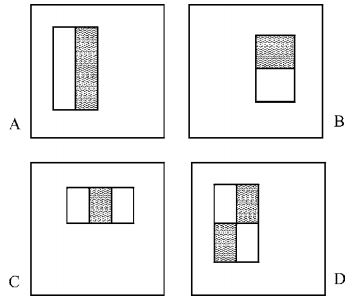
\includegraphics{haar.JPG}
		\caption[Exemple de 4 caractéristiques de Haar]{Exemple de 4 caractéristiques de Haar (source: \citep{VIO})}
		\label{fig:haar}
	\end{figure}
	
Le calcul d'une caractéristique de Haar requiert des accès aux valeurs de tous les pixels de la zone rectangulaire considérée. Quand le rectangle est de grande dimension, le calcul de la caractéristique devient contraignant temporellement. Pour pallier à cela, on fait appel à l'image intégrale ; Elle rend constant le calcul d'une caractéristique de Haar à n'importe quelle échelle.

L'image intégrale à l'emplacement $(x, y)$ dans une image contient la somme des images élémentaires au-dessus et à gauche de $(x, y)$ inclus : 
  \[ii(x, y)=\sum_{x'< x, y'< y }{i(x', y')}\] où $ii(x, y)$ est l'image intégrale et $i(x, y)$ l'image d'origine (voir figure \ref{fig:integr} ). 
	\begin{figure}[htbp]
		\centering
			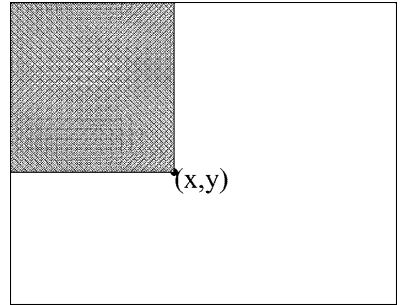
\includegraphics[height=175pt, width=175pt]{integr.JPG}
		\caption{image intégrale au point (x,y)}
		\label{fig:integr}
	\end{figure}
	
L'image intégrale est calculée rapidement en utilisant la paire de récurrences ci-dessous.
 \begin{eqnarray*}
s(x,y)=s(x,y-1)+i(x,y)\\
ii(x,y)=ii(x-1,y)+s(x,y)
\end{eqnarray*}
où $s(x,y)$ est la somme cumulative  des pixels sur une ligne. On a $s(x,-1)= 0$ et  $ii(-1,y) =0$.


Dans l'image intégrale, chaque pixel a pour valeur la somme des pixels se trouvant dans le rectangle supérieur gauche de l'image et lui même. Le calcul de la somme des valeurs des pixels d'une zone rectangulaire se fait en accédant seulement à quatre pixels de l'image qui sont les sommets de la zone rectangulaire. Soit la figure \ref{fig:rect} ci-dessous représentant une image intégrale.
\begin{figure}[htbp]
	\centering
		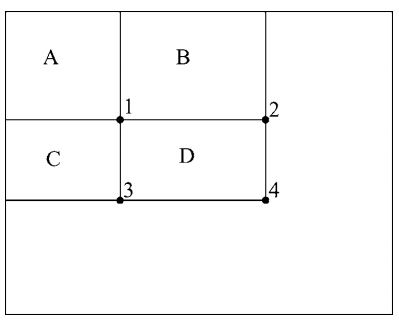
\includegraphics[height=175pt, width=175pt]{rect.JPG}
	\caption{calcul de la somme des pixels d'un rectangle}
	\label{fig:rect}
\end{figure}
Pour calculer la somme des pixels dans le rectangle D, on utilise uniquement les valeurs des pixels aux positions 1, 2, 3 et 4. La valeur du pixel en 1 est la somme des pixels du rectangle A. La valeur à la position 2 est A+B, à la position 3, elle est A+C, et à la position 4 elle est A+B+C+D. Ainsi on a : 
\begin{eqnarray*}
			4+1  & = &A+B+C+D+A \; (\; on\;  ajoute\;  A \; membre\;  à\;  membre\; )\\
			4+1  & = &2+3+D  \; (\; \; on \; réduit )\\
      D    & = &4+1-(2+3)\; (\; on\; tire D )
\end{eqnarray*}
														

	\subsubsection{Algorithme d'apprentissage basé sur Adaboost}
Pour localiser les visages sur l'image d'entrée, cette dernière est scannée par une fenêtre de dimension déterminée. La fenêtre parcourt l'image et son contenu est analysée pour vérifier l'existence ou non d'un visage. La classification est faite à l'aide des caractéristiques de Haar extraites de l'image et pour faciliter l'analyse, l'image est mise sous sa forme intégrale. Mais, pour une fenêtre de $24 \times 24$ pixels il y a 45 396 caractéristiques de Haar \citep{VIO}, les traiter toutes prendrait beaucoup trop de temps pour une application en temps réel. Pour surmonter ce problème, une variante de la méthode de boosting Adaboost est utilisée.

Je présente ci-dessous la méthode Adaboost ainsi que sa variante qui constitue le second apport de Viola et Jones.

Adaboost est une méthode d'apprentissage permettant de "booster" les performances d'un classifieur quelconque nommée "classifieur faible". L'idée est de faire passer les candidats à classifier à travers plusieurs classifieurs faibles, chacun étant entraînée en portant plus d'attention sur les candidats mal classifiées par le classifieur précédent.

Pour cela, des poids sont associées aux échantillons du training set

$((x_i; y_i) i = 1,\ldots ,m)$, tout d'abord de manière équilibrée :  


	\subsubsection{Cascade}
	
	Parmi l'ensemble des états de la fenêtre de recherche (c'est-à-dire les candidats) une partie peut être éliminée sur la base de l'évaluation de quelques caractéristiques de Haar : d'où le concept de cascade. Après élimination, les candidats restants sont analysés par des classifieurs forts, plus complexes demandant un plus grand temps de traitement. Cette manière de procéder évite donc d'effectuer des analyses lourdes en temps de calcul sur des échantillons pour lesquels il est rapidement possible de se rendre compte qu'ils sont négatifs. La classification apparaît donc comme une succession d'étapes où les échantillons classifiés positifs passent à l'étape suivante et les échantillons négatifs sont éliminés (voir figure \ref{fig:cacasde}).
	
	\begin{figure}[htbp]
		\centering
			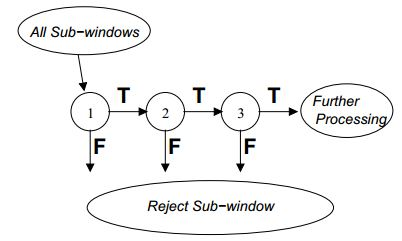
\includegraphics{cacasde.JPG}
		\caption[cascade de classifieurs forts]{cascade de classifieurs forts (source\citep{VIO})}
		\label{fig:cacasde}
	\end{figure}
	
	L'inconvénient de ce processus en cascade est que si le premier étage rejette un faux négatif, alors il ne sera plus jamais récupéré par la cascade. En d'autres termes le visage ne sera jamais détecté. Par contre si le premier étage transmet un faux positif, il pourra toujours être éliminée
aux étages suivants de la cascade.

Pour que la localisation soit rapide et atteigne des taux de détection élevés, les paramètres comme le nombre d'étages dans la	 cascade, leurs seuils de détection $\theta$ et le nombre de caractéristiques T considéré à chaque étage doivent être choisis convenablement. Ce choix doit être effectué pendant la construction de la cascade. 

L'entraînement de la cascade implique deux types de compromis : un classifieur avec un grand nombre de caractéristiques aura un taux élevé de détection et un faible taux de faux positifs, mais exigera un grand temps de calcul. Construire un classifieur avec le plus petit nombre possible d'étages dans la cascade, un nombre raisonnable de caractéristiques dans chaque étage et un meilleur taux de détection à chaque étage serait l'idéal. Malheureusement construire un tel classifieur reste un problème très difficile à résoudre.

Dans l'entraînement, une structure très simple est utilisée pour produire un classifieur effectif et très efficace. Chaque étape dans la cascade réduit le taux de faux positifs et diminue le taux de détection. Une cible est sélectionnée pour la réduction minimum des faux positifs et la baisse maximale de la détection. Chaque étape est entraînée en ajoutant des caractéristiques jusqu'à ce que la cible et les taux de faux positifs soient rencontrés (ces taux sont déterminés en testant le détecteur sur un ensemble de la validation). Les étapes sont ajoutées jusqu'à ce que la cible totale pour les faux positif et le taux détection soit rencontrée.

Le détecteur de visage développé par Viola et Jones dans \citep{VIO} est constitué de 38 étages et de plus de 600 caractéristiques. Néanmoins, elle opère rapidement. Sur un dataset difficile, contenant 507 visages et 75 millions de sous-fenêtres, les visages sont détectés après évaluation de 10 caractéristiques en moyenne  par sous-fenêtre. Ce système est approximativement 15 fois plus vite qu'une mise en œuvre du système de détection construit par Rowley et al. dans \citep{Row}.
Le tableau ci-dessous montre les performances de quelques algorithmes de détection de visage sur la base de données d'images MIT+CMU \footnote{MIT+CMU est une base de 130 images et 507 visages}.
 
\begin{table}[htbp]
	\centering
		\begin{tabular}{|l|c|c|c|c|c|c|c|}
			\hline	\backslashbox{d\'{e}tecteur}{faux positifs} & 10 & 31 & 50 & 65 & 78 & 95 & 167 \\
			\hline  Viola-Jones       & 76.1\% & 88.4\% & 91.4\% &92.0\% &92.1\%& 92.9\% &93.9\% \\
			\hline	Viola et Jones (Voting)& 81.1\% & 89.7\% & 92.1\% &93.1\% &93.1\%& 93.2\% &93.7\% \\
			\hline	Rowley-Baluja-Kanade   & 83.2\% & 86.0\% & -& - & - & 89.2\% & 90.1\%\\
			\hline	Schneiderman-Kanade     & - & -& - & 94.4\% & - & -  & -\\	
			\hline	Roth-Yang-Ahuja     & - & -& - & - & 94.8\%  &-   & -\\	
			\hline
		\end{tabular}
	\caption[taux de détection pour différents nombre de faux positifs sur la base d'image MIT+CMU]{taux de détection pour différents nombre de faux positifs sur la base d'image MIT+CMU}
	\label{tab:tauxDeDétection}
\end{table}
\subsection{Travaux améliorant l'algorithme de Viola et Jones}
\subsubsection{Nouvelle représentation intégrale}
  En plus de la représentation intégrale présentée plus haut, Lienhart et al. ont proposé une représentation intégrale inclinée où chaque pixel a pour valeur la somme des valeurs des pixels compris dans la zone rectangulaire inclinée de 45\degres dont le point extrême droit est le pixel considérée. Aux modèles initiaux de Viola et Jones sont donc ajoutés leurs équivalents inclinés de 45\degres. Les auteurs ont ainsi obtenu des améliorations de l'ordre d'un demi-pourcent.
	
	\begin{figure}[htbp]
		\centering
			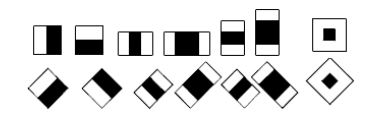
\includegraphics{haaram.JPG}
		\caption[représentation intégrale inclinée]{représentation intégrale inclinée (source : \cite{MAT}) }
		\label{fig:haaram}
	\end{figure}
	
	\subsubsection{Améliorations du Training set}
	Ayant constaté que l'on pouvait améliorer les performances du classifieur en préparant le set d'entraînement, Chen et al. \citep{CHEN} proposent une méthode basée sur un algorithme génétique pour étendre le set de visages. Selon eux leur approche est la plus prometteuse  dans le domaine de l'optimisation du Training set.
	
\section{Méthodes de reconnaissance de visages}

Une multitude de techniques de reconnaissance de visage ont été développées ces vingt dernières années.  L'identification  de  visage  est  un  axe  de  recherche  ouvert  attirant  des  chercheurs venants  de  disciplines  différentes  :  psychologie,  reconnaissance  de  formes, réseaux neuraux, vision artificielle et infographie. Le but ultime de la reconnaissance automatique de visage est  de  rivaliser,  voir  même  dépasser,  les  capacités  humaines  de reconnaissance. Nous allons détaillé dans cette partie quelques méthodes de reconnaissance faciale.

\subsection{Méthodes globales ou holistiques}
Les méthodes globales sont celles qui identifient un visage en prenant l'image entière de ce dernier comme entrée du système de reconnaissance \citep{Sou12}. Chaque image de visage de dimension $(n,m)$ est représentée 
par un vecteur simple de dimension $n\times m$, en concaténant les valeurs du niveau de gris de tous les pixels  de l'image du visage. L'avantage de cette représentation est qu'elle préserve implicitement les informations de texture et de forme nécessaire pour la reconnaissance de visages, mais nécessite une grande dimension de l'espace image. 

Ainsi, une image $100\times 100$, par exemple, est représentée par un vecteur de dimension $10^4$. Or le nombre d'images d'apprentissage pour chaque personne doit être au moins égal à dix fois la dimension du vecteur \citep{Jai}, il faut $10^5$ images  par  personne, ce qui serait difficilement réalisable en pratique.  Des techniques de réduction de  dimension sont généralement employées. Je présente ci-dessous les techniques de réduction par ACP et ADL.

\subsubsection{Analyse en Composante Principale (ACP) }

L'algorithme  PCA (Principal Component Analysis) est né des travaux de M. Turk et P. Pentland au MIT Media 
Lab, en 1991\citep{TURK}. L'ACP est une méthode mathématique qui peut être utilisée pour simplifier un ensemble de données en réduisant sa dimension. Elle permet ainsi de représenter efficacement les images de visage, qui peuvent approximativement être reconstruites à partir d'un petit ensemble de poids et d'une image de visage standard. Ces poids sont obtenus en projetant l'image du visage dans un espace de visage engendré par les visages propres.

La méthode \og eigenface \fg{} est l'une des méthodes basées sur l'ACP les plus utilisées \citep{Sou12}. Son principe est le suivant : étant donné un ensemble d'images de visages exemples, il s'agit tout d'abord de trouver les composantes principales de ces visages. Les visages propres (eigenfaces) sont des visages de même taille que les images d'apprentissage et qui montrent des visages ayant un aspect assez particulière (voir figure \ref {fig:eigenface}). Du point de vue mathématique, il s'agit des composantes principales de la distribution des visages, ou les vecteurs propres (eigenvectors) de la matrice de covariance de l'ensemble des images du visage. Chaque image du training set peut être représenté comme combinaison linéaire des visages propres et du visage moyen \citep{TOLBA}.
\begin{figure}[htbp]
	\centering
		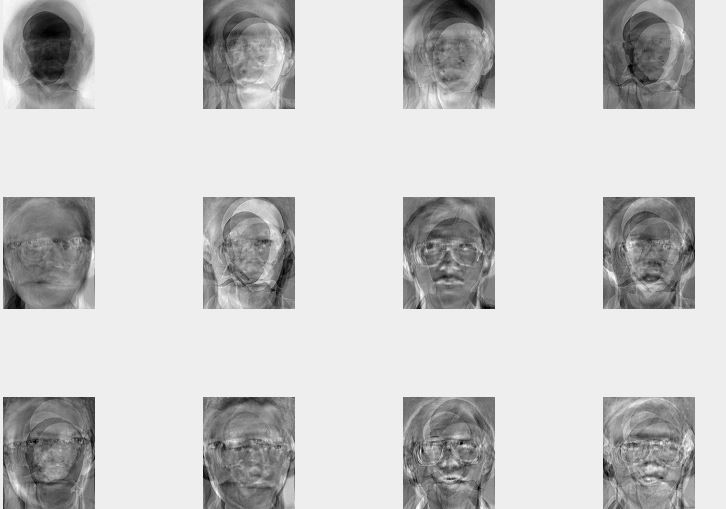
\includegraphics[height=250pt, width=400pt]{eigenface.JPG}
	\caption{exemple de faces propres}
	\label{fig:eigenface}
\end{figure}

Le nombre de visages propres est égal au nombre de visage dans le training set. Néanmoins, on peut réduire les calculs en ne considérant que les "meilleurs" eigenfaces (les meilleurs eigenfaces sont ceux ayant les plus larges valeurs propres qui représentent la plupart de variance dans l'ensemble des images de visage). L'ensemble  
de ces meilleurs eigenfaces forme le " Low Dimensional Space".
Le nombre d'images d'apprentissage influence sur les performances de l'algorithme eigenfaces. Pour illustrer cela, Wang et al. dans \citep{WAN} ont utilisé la base de données ORL\footnote{La base de données ORL 
contient des images de 40 individus, chacun étant enregistré sous 10 vues différentes.} comme base de test. Il ressort de leur étude que les performances de la méthode eigenface baisse avec la diminution du nombre d’exemples d'apprentissage pour chaque personne.  Dans le cas extrême, si le training set contient seulement une image, le taux d'identification moyen de l'eigenface tombe en dessous de 65 \%. Ce taux atteint 95\% quand on utilise neuf exemples d'apprentissage par personne. 


\subsubsection{Processus de reconnaissance par Eigenfaces}
Le processus de reconnaissance s'effectue en deux phases : la phase d'apprentissage et la phase de vérification.
La phase d'apprentissage  comprends dans l'ordre : 

\begin{itemize}
	\item [\textbullet]l'acquisition, la lecture et la normalisation des images des visages d'apprentissages (de taille R),
	\item [\textbullet]le calcul du visage moyen de ces images,
	\item [\textbullet]la détermination de la matrice de covariance $L=S^tS$ où $S$ est une matrice dont les colonnes sont les images obtenues après soustraction du visage moyen de chaque visage d'apprentissage normalisée,
	\item [\textbullet]le calcul des vecteurs propres $V$ et des valeurs propres $D$ de la matrice de covariance,
	\item [\textbullet]le calcul des visages propres (eigenfaces) selon la formule $U=S\times V\times (abs(D))^\frac{-1}{2}$,
	\item [\textbullet]Enfin le calcul des poids des visages de la base (de taille M) en les projetant dans le sous-espace engendré par les visages propres.
\end{itemize} 
   
Pendant la phase de vérification, on fait l'acquisition, la lecture et la normalisation de l'image de vérification (de taille R). Puis on soustrait le visage moyen de l'image normalisée. Ensuite on calcule le poids de l'image en utilisant les images propres comme une base de projection. Enfin on mesure la similarité en utilisant la distance euclidienne. %\citep{}.

L'ACP est une technique rapide, simple et populaire dans l'identification de modèle, c'est l'une des meilleures techniques. Cependant, l'ACP n'est pas optimisée pour la séparabilité (discrimination) de classe aux dépens de l'analyse discriminante linéaire (LDA). 

\subsubsection{Analyse Discriminante Linéaire (ADL)}

L'algorithme LDA est né des travaux de Belhumeur et al. De Yale University (USA), en  1997 \citep{BEL}. Il est aussi connu sous le nom de \og Fisherfaces \fg{}. Les méthodes basées sur l'Analyse Discriminante Linéaire  déterminent les directions de projection les plus discriminantes dans l'espace engendré par les visages propres. Pour cela, elles maximisent les variations inter-personne par rapport aux variations intra-personne. Pour utiliser la technique LDA, l'on doit préalablement organiser la base d'apprentissage en plusieurs classes : en raison d'une classe par personne et plusieurs images par classe.  La LDA analyse les vecteurs propres de la matrice de dispersion des données, avec pour  objectif de maximiser les variations entre les 
images d'individus différents (interclasses) tout  en minimisant les variations entre les images d'un même individu (intra-classes). Cependant, si un seul exemple d'apprentissage par personne est utilisé, c'est-à-dire
si les variations intra classes nulles, alors les performances de l'ADL deviennent faibles par rapport à celles  qui sont données par l'eigenface \cite{MAR}.

Plusieurs autres méthodes ont été développées ces dernières années à l'instar de la méthode eigenface probabiliste, la méthode de la Machine Vecteur Support (SVM), la méthode de la ligne caractéristique, la méthode Laplacianfaces. Ces méthodes sont généralement plus performantes que la méthode eigenface basique \cite{Sou12}, mais lorsque le training set est constitué d'une seule image, certaines de ces méthodes se réduisent à l'eigenface basique ou peuvent ne plus fonctionner.

Les méthodes holistiques souffrent du problème du petit nombre d'échantillon (small size sample problem)qui dégrade leurs performances. Néanmoins des méthodes surmontant ce défaut comme (PC)$^2$A \citep{WU}, sa généralisation E(PC)$^2$A \cite{SONG} et la 2DPCA \citep{JIAN} ont été développées. Des stratégies visant à étendre le training set peuvent être également utilisées (utilisation des images symétriques gauches et droites pour générer de nouvelles vues, la méthode de déformation parallèle pour générer de nouvelles poses à partir d'une première photo). 
\subsection{Méthodes locales}
Les méthodes locales utilisent les caractéristiques faciales locales pour la reconnaissance de visage. Cette catégorie se divise en deux sous-catégories basées respectivement sur des caractéristiques et des apparences locales.
\subsubsection{Méthodes basées sur l'apparence locale}

Les méthodes basées sur l'apparence locale utilisent en entrée plusieurs vecteurs correspondant aux caractéristiques du visage à reconnaître. Elles sont utilisées de manière modulaire pour les différentes régions du visage. Un modèle global est alors défini par la combinaison de plusieurs modèles locaux. De cette façon, les différentes régions du visage ne sont pas affectées de la même manière par les différentes sources de vulnérabilités. Ces méthodes sont à priori mieux adaptées pour le problème à échantillon
unique \cite{XIAO}.
\subsubsection{Méthodes basées sur des caractéristiques locales}
Les méthodes basées sur les caractéristiques locales peuvent être classées en deux catégories: les approches géométriques et les approches basées sur les graphes.

Pour des approches géométriques, des propriétés géométriques sont extraites à partir de la localisation de points clés sur le visage (tel que le nez, la bouche et les yeux).
Un exemple est le système décrit par Brunelli et Poggio \citep{BRU}  qui extrait automatiquement 35 caractéristiques géométriques du visage et qui utilise les classifieurs de Bayes pour calculer la similitude. Pour ce système, les auteurs ont enregistré un taux d'identification de 90\% sur une base de données de 47 sujets. Le  coût  de  stockage  des  techniques géométriques est très bas comparé à celui des autres techniques. Toutefois, les méthodes purement géométriques présentent deux principaux inconvénients qui sont :
\begin{itemize}
	\item la localisation des points clés qui n'est pas toujours chose facile lorsque les occlusions ou variations d'expressions ou de pose surviennent,
	\item  l'information nécessaire à une reconnaissance robuste n'est pas forcement contenue dans ces quelques points clés.
\end{itemize}

Comme exemple de méthodes locales, nous avons la méthode des Local Binary Patterns, la méthode EBGM \cite{EBGM} (Elastic Bunch Graph Matching), etc.

Le tableau ci-dessous (tirée de \cite{Sou12}) est une comparaison entre les méthodes basées sur les deux types de caractéristiques.
\begin{table}[htbp]
	\centering
		\begin{tabular}{|l|l|l|}
			\hline
			Facteurs de variation & Caractéristiques locales& Caractéristiques globales\\
			\hline illuminations & très sensible& sensible\\
			\hline expressions & pas sensible& sensible\\
			\hline pose & sensible& très sensible\\
			\hline bruit & très sensible& sensible\\
			\hline occlusions & pas sensible& très sensible\\
			\hline
		\end{tabular}
	\caption{comparaison des méthodes basées sur les caractéristiques globales ou locales} 
	\label{tab:comparaison}
\end{table}
\subsection{Méthodes hybrides}
Comme leur nom indique, les méthodes hybrides sont celles qui combinent les méthodes globales et locales. Le but est de bénéficier des avantages de l'un et de l'autre. La combinaison efficace entre caractéristiques locales et globales reste pour le moment un problème et peu de travaux sur son application au problème de la reconnaissance faciale existent \citep{XIAO}.

Le tableau \ref{tab:scoresDeCertaines} extrait de \cite{Beymer}montre les performances des méthodes les plus performantes dans le domaine de la reconnaissance faciale à partir d'une seule image par personne.

\begin{table}[htbp]
	\centering
		\begin{tabular}{|l|p{2cm}|p{1cm}|p{1cm}|p{2cm}|p{3cm}|}
			\hline
			\footnotesize méthode&\footnotesize BD d'images& \footnotesize personnes de test&\footnotesize images de test& \footnotesize score le plus élevé/score de base& \footnotesize facteurs de variation \\ \hline
		\footnotesize Parallel deformation&\footnotesize N/A&62&620&\footnotesize 85.0/ 32.1&\footnotesize Pose\\ \hline
		\footnotesize Local probalistic subspace& \footnotesize AR&100&600&\footnotesize 82.5/ 70.2& \footnotesize Expression, temps\\ \hline
		\footnotesize Someface& \footnotesize AR&100&600&\footnotesize 93.7/ 70.2&\footnotesize Expression, temps\\ \hline
			\footnotesize 2DPCA& \footnotesize AR&100&600& \footnotesize 74.8/ 70.2&\footnotesize Expression, temps\\ \hline
			\footnotesize ID-DDHM&\footnotesize AR&120&1440&\footnotesize 89.8/ 27.2&\footnotesize Expression, illumination, temps\\ \hline
			\footnotesize (PC)$^2$A&\footnotesize FERET&200&200&\footnotesize 83.5/83.0&\footnotesize N/A\\ \hline
		\footnotesize E(PC)$^2$A&\footnotesize FERET&200&200&\footnotesize 85.5/ 83.0&\footnotesize N/A\\ \hline
		\footnotesize SDV perturbation&\footnotesize FERET&200&200&\footnotesize 85.0/ 83.0&\footnotesize N/A\\ \hline
		\footnotesize Modular FLDA&\footnotesize FERET&200&200&\footnotesize 86.5/ 83.0&\footnotesize N/A\\ \hline
		\footnotesize Component LDA&\footnotesize FERET&70&350&\footnotesize 78.6/ 32.0&\footnotesize Expression, illumination, temps\\ \hline
		\footnotesize EBGM&\footnotesize FERET&1196&1196&\footnotesize 95.0/ 79.7&\footnotesize Expression\\ \hline
		\footnotesize LBP&\footnotesize FERET&1196&1196&\footnotesize 97.0/ 79.7&\footnotesize Expression\\ \hline
		\footnotesize Discriminant PCA&\footnotesize FERET&256&914&\footnotesize 72.0/ 74.0&\footnotesize Expression,temps\\ \hline
		\footnotesize Analytic-to-hilistic approch&\footnotesize ORL&40&160&\footnotesize 84.0/ 74.7&\footnotesize Pose\\ \hline
		\footnotesize face specific subspace&\footnotesize Yale&15&150&\footnotesize 95.3/74.7&\footnotesize Expression,illumination\\ 
			\hline
		\end{tabular}
	\caption[algorithmes et leurs performances sur le 'one sample problem']{scores de certaines méthodes s'attaquant au problème de la reconnaissance faciale avec des training sets composés d'un seul échantillon par personne}
	\label{tab:scoresDeCertaines}
\end{table}


\section{Conclusion} 
Dans ce chapitre, nous avons présenté un ensemble de techniques de détection et de reconnaissance de visages. L'
engouement  pour  les  systèmes  de  reconnaissance  des  visages  est  justifié  par  les  nombreux
avantages de cette approche.

\chapter[\small LA RECONNAISSANCE FACIALE PAR LES M\'{E}THODES EIGENFACE ET LBP]{LA RECONNAISSANCE FACIALE PAR LES MÉTHODES EIGENFACE ET LBP}
\section{Introduction}
La reconnaissance de visage est sans doute le moyen le plus utilisé au quotidien pour identifier un  membre de son entourage. La reconnaissance automatique de visage s'inscrit dans le domaine vaste la de vision par ordinateur qui part du constat selon lequel le sens le plus utilisé chez l'homme est la vue. Dès lors, il peut s'avérer important de \og donner les yeux à son ordinateur\fg{} : ainsi il pourra remplacer l'homme dans les tâches répétitives de reconnaissance faciale. Parmi les différentes méthodes présentées au chapitre précédent, certaines ont l'avantage d'être rapide, facile à mettre en œuvre ou ont un taux élevé de reconnaissance. Dans ce chapitre, nous présentons dans un premier temps la méthode de reconnaissance eigenface, puis dans un second temps l'approche LBP(Local Binary Patterns). 
\section{Reconnaissance par eigenface}

\subsection{présentation de la méthode eigenface}
L'algorithme PCA ou eigenface s'appuie sur des propriétés statistiques et utilise l'algèbre linéaire pour classifier les visages. C'est l'un des algorithmes les plus utilisés car il est relativement facile à mettre en œuvre et est à la base de nombreux autres algorithmes. Ses principaux inconvénients c'est sa sensibilité aux problèmes d'éclairage, de pose et d'expressions faciales.

L'approche eigenface consiste à représenter un visage $\Phi_{i}$ comme une combinaison linéaire d'un ensemble d'images 
M, ces dernières formant ainsi une base de référence. Mathématiquement, cela revient à établir l'équation \ref{eq5} : 
\begin{eqnarray}
\Phi_{i}=\sum_{i=1}^{n}{p_id_i}
\label{eq5}
\end{eqnarray}
où $d_i$ représente le visage propre, et $p_i$ le coefficient associé.

Pour calculer les $p_i$ représentant les poids, on traite une image $I_i(m,n)$ comme un vecteur $\Gamma_(m\times n,1)$ dans un espace vectoriel de plus grande dimension $N=m \times n$, par concaténation de colonnes.

\[
   I_i(m,n)=\begin{pmatrix}
\alpha_{11} & \alpha_{12}& \ldots & \alpha_{1n}\\
\alpha_{21} & \alpha_{22}& \ldots & \alpha_{2n}\\
\ldots& \vdots& \vdots & \vdots        \\
\alpha_{m1} & \alpha_{m2}& \ldots & \alpha_{mn}
\end{pmatrix}\]

est transformée en

\[\Gamma_i(m\times n,1)= \begin{pmatrix}
\alpha_{11} \\
\alpha_{12} \\
\vdots     \\
\alpha_{1n}   \\
\alpha_{21}   \\
\alpha_{22}  \\
\vdots   \\
\alpha_{2n}  \\
\vdots        \\
\alpha_{m1} \\
\alpha_{m2}\\
\vdots \\
\alpha_{mn}
\end{pmatrix} 
\]
Les coefficients $\alpha_{i,j}$ représentent les valeurs des pixels en niveau de gris, codés de 0 à 255.
On peut alors rassembler les M images d'apprentissage dans une unique matrice, nous obtenons une matrice d'images $\Gamma$, où chaque colonne représente une image $\Gamma_i$.
\[\Gamma= \begin{pmatrix}
\alpha_{11} &\beta_{11} &\ldots&\zeta_{11}\\
\vdots      &\vdots     &\ldots&\vdots\\
\alpha_{1n} &\beta_{1n}&\ldots&\zeta_{1n} \\
\alpha_{21} &\beta_{21} &\ldots&\zeta_{21} \\
\vdots      &\vdots     &\ldots& \vdots  \\
\alpha_{2n} &\beta_{2n} &\ldots&\zeta_{2n} \\
\vdots      & \vdots    &\ldots&\vdots    \\
\alpha_{m1} &\beta_{m1} &\ldots&\zeta_{m1} \\
\vdots      &\vdots     &\ldots&\vdots \\
\alpha_{mn} &\beta_{mn} &\ldots&\alpha_{mn}
\end{pmatrix} 
\]

On peut alors déduire le visage moyen par la formule 
\begin{eqnarray}
\Psi=\frac{1}{M}\sum_{i=1}^{M}{\Gamma_i}
\label{eq6}
\end{eqnarray}
A chaque visage d'apprentissage, on soustrait le visage moyen de la manière suivante.
\begin{eqnarray}
\phi_i=\Gamma_i -\Psi
\label{eq7}
\end{eqnarray}
$i=1, 2,\ldots, M$ où $\phi_i$ représente le $i^{ème}$ visage auquel on a soustrait le visage moyen.

 On obtient alors les informations propres à ce visage. Dès lors on peut calculer la matrice de covariance D. Elle correspond à
\begin{eqnarray}
D=QQ^{t}
\label{eq8}
\end{eqnarray}
où $Q=\begin{pmatrix} \phi_1&\phi_2 &\ldots&\phi_M\end{pmatrix}$.

L'étape suivante est le calcul des valeurs propres $d_i$ de la matrice $D$. Comme la matrice $D$ est carrée d'ordre $n\times m$, on aura également $n\times m$ vecteurs propres de dimension $n\times m$ chacun. Il peut s'avérer difficile et très long de les calculer. La solution consiste à réduire la dimension de l'espace de travail. Nous allons donc considérer la matrice $E=Q^tQ$ et trouver ses valeurs propres. Par  exemple \citep{SAB}, pour 50 images de résolution $180\times200$, nous pourrions résoudre une  matrice L de $50\times50$ au lieu d'une matrice de $36000\times 36000 $ pour ensuite prendre les  combinaisons  linéaires  appropriées  des  images $\phi_i$. Cette opération permet de passer d'une complexité de l'ordre du nombre de pixel de l'image à une complexité de l'ordre du nombre d'image. Le passage de la matrice D à la matrice E est justifié par le fait que les vecteurs propres de ces deux matrices sont liés de manière assez proche.

En effet 
\begin{eqnarray}
Ee_i=Q^tQe_i=\lambda_ie_i
\label{eq9}
\end{eqnarray}
avec $\lambda_i$ la valeur propre associé au vecteur propre $e_i$.\\
En multipliant l'équation \ref{eq9} par la matrice Q, il ressort :
\begin{eqnarray}
QEe_i=QQ^tQe_i
\label{eq10}
\end{eqnarray}
soit \begin{eqnarray*}
QEe_i=DQe_i=Q\lambda_ie_i
\label{eq11}
\end{eqnarray*}
Donc si $e_i$ est un vecteur propre de la matrice E associé à une valeur propre $\lambda_i$, alors $Qe_i$ est un vecteur propre de la matrice D associé à la même valeur propre $\lambda_i$. Ainsi, nous avons $d_i$ vecteur propre de D, avec \begin{eqnarray}
d_i = Qe_i
\label{eq12}
\end{eqnarray}
Nous pouvons donc trouver les valeurs propres de l'énorme matrice D en trouvant 
d'abord les valeurs propres de la matrice E beaucoup plus petite, puis pour trouver les vecteurs propres de D, il suffit juste de multiplier les vecteurs propres de E par la matrice Q. Une fois les vecteurs propres trouvés, on les classe selon leurs valeurs propres associées et de manière décroissante. Puisque les valeurs propres les plus grandes renferment le plus d'informations, on va sélectionner les k meilleures valeurs propres (les plus significatifs). On définit alors un espace vectoriel engendré par ces $k$ vecteurs propres, que 
l'on appelle l'espace des visages $E_v$ ou \og Face Space\fg{}. Une image originale est alors un vecteur de cette espace vectoriel(c'est-à-dire s'écrit comme combinaison linéaire des vecteurs propres). La figure \ref{fig:eigenface} montre un exemple de faces propres.

Dans la pratique, on choisit k selon un pourcentage $\gamma$ tel que
\begin{eqnarray}
\frac{\sum_{i=k+1}^{n}\lambda_i}{\sum_{i=1}^{n}\lambda_i} < \gamma
\label{eq13}
\end{eqnarray}
où $n$ représente le nombre total de valeurs propres.
Les \og k \fg{} premiers vecteurs propres correspondant aux \og k \fg{} plus grandes valeurs doivent être convenablement choisies car constituent un paramètre  critique  sur  lequel  dépend  la  performance  du  système  de reconnaissance. 
\subsection{Processus de reconnaissance par eigenface}
Pour classifier un visage par eigenface, on projecte d'abord les images d'apprentissage sur l'espace des visages $E_v$. Une image $\Gamma_i$ est alors transformée en ses \og composantes Eigenfaces\fg{} par une simple opération de projection vectorielle.
 \begin{eqnarray}
p_i&=&d_i^t\phi_i\\
   &=&d_i^t(\Gamma_i -\Psi)
\label{eq14}
\end{eqnarray}pour $i=1,2, \ldots, k$.

Les  vecteurs $p_i$ sont  appelés  vecteurs  de  poids  et  forment  une  matrice 
$\Pi=\begin{pmatrix} p_1&p_2 &\ldots& p_k\end{pmatrix}$  qui  décrit  la  contribution  de  chaque  eigenface  dans  la  représentation  de l'image  d'entrée. La  matrice $\Pi$ est  alors  utilisée  pour  trouver  quelle  est,  parmi  un  nombre 
prédéfini de classes, celle qui décrit le mieux une image d'entrée.

La méthode la plus simple pour déterminer quelle classe de  visage fournit la meilleure
description d'une image d'entrée est de trouver la classe de visage $k$ qui minimise la distance euclidienne.
\begin{eqnarray}
\epsilon_k^2=\left\|\Pi-\Pi_k\right\|
\label{eq15}
\end{eqnarray}
Les étapes suivantes résume la techniques d'eigenfaces.

La phase d'apprentissage comprends :


\begin{itemize}
	\item [\textbullet] la collecte  des  M  images  faciales  et  construction  de  la  matrice  $\Gamma$, par concaténation des colonnes des images faciales. 
		\item [\textbullet]  le calcul du visage moyen en sommant les colonnes de la matrice $\Gamma$ et en divisant le vecteur résultant par le nombre d'image d'entrée M ( voir \ref{eq6}).
     \item [\textbullet] la soustraction du visage moyen de la matrice $\Gamma$ pour obtenir la matrice $Q$ ; où chaque élément représente la variance des valeurs d'intensité de chaque pixel.
		\item [\textbullet] le calcul de la matrice $E=Q^tQ$,
		\item [\textbullet] le calcul des vecteurs propres de $E$ puis leur tri dans un ordre descendant selon les valeurs propres associées.
		\item [\textbullet] le calcul  des  vecteurs  propres  de  la  matrice  de  covariance $C^t$  et  obtention  des  visages propres en multipliant les vecteurs propres de $E$ par la matrice $Q$.
		\item [\textbullet] le choix des $k$ meilleurs valeurs propres et les vecteurs propres associés.
		\item [\textbullet] la détermination du poids des images d'entrée en projetant chaque image dans l'espace
visage.
\item [\textbullet] la sauvegarde du visage moyen, les eigenfaces et la matrice de projection (de poids) des images.
\end{itemize}

Les 9 étapes ci-dessus transforment une base de données images en un ensemble de projection dans l'espace visage.

L'étape de reconnaissance comprends : 
\begin{itemize}
	\item [\textbullet] le prétraitement de l'image d'entrée et soustraction du visage moyen,
	\item [\textbullet] la détermination du poids de l'image d'entrée par la projection de celle–ci dans l'espace 
visage en multipliant le vecteur résultant de la première étape d'apprentissage par les eigenfaces de la base de données.
  \item [\textbullet]la mesure de la similarité  en  utilisant  des  métriques  telles  que  la  distance euclidienne.
	\end{itemize}
	
	NB. Plusieurs métriques peuvent être utilisés pour mesurer la similarité de deux vecteurs $X=(x_1,x_2,\ldots,x_n)$ et $Y=(y_1,y_2,\ldots,y_n)$ à l'instar de la distance euclidienne $$d(X,Y)=\sqrt{\sum_{i=1}^{n}{\left|x_i-y_i\right|^2}}$$ la distance de City-Block (ou de Manathan) $$d(X,Y)=\sum_{i=1}^{n}{\left|x_i-y_i\right|}$$ la distance de Mahalanobis (cf. \cite{KATO}).
	
	Toutefois, le choix de la mesure est parfois difficile et est souvent argumenté par rapport à l'espace d'attributs.
	
\section{Reconnaissance par la méthode des Local Binary Patterns} 
\subsection{Présentation de la méthode LBP}
La méthode LBP telle que décrite par Ahonen et al. dans \cite{TIM} prend en entrée un carré de  9 pixels et a pour sortie un nombre binaire 8 bits. Les auteurs ont été motivés par le fait qu'un visage peut être vu comme un assemblage de micro-patterns dont la description par LBP est à la fois bonne, robuste face aux variations de gris et rapide à générer. 

\begin{figure}[htbp]
	\centering
		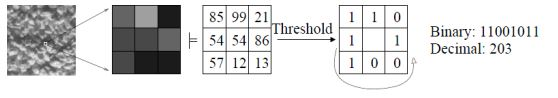
\includegraphics{BLP.JPG}
	\caption[opérateur LBP ]{opérateur LBP \textit{(source :\cite{TIM})}}
	\label{fig:LBP}
\end{figure}

Un seuil est appliqué tel que tous les pixels périphériques dont la valeur est supérieure à la valeur du pixel central se voient attribuer la valeur 1 tandis que les autres reçoivent la valeur 0. La valeur LBP est obtenue en lisant autour du pixel central dans le sens trigonométrique (comme indiqué dans la figure \ref{fig:LBP}. Pour convertir toute l'image, on déplace le carré de conversion $3\times 3$ sur l'ensemble de l'image.

Pour rester fiable, l'opérateur LBP a été étendue.  Dans ce cas, un cercle de rayon R autour du pixel central et les valeurs des P points échantillonnés sur le bord de ce cercle sont prises et comparées avec la valeur du pixel central (voir figure \ref{fig:lbpam} tirée de \cite{TIM} ). Cet entourage sera notée $(P,R)$. Comme ces P points ne tombent pas nécessairement
au centre d'un pixel de l'image, leurs valeurs sont obtenues par interpolation bilinéaire \cite{TIM}.
\begin{figure}[htbp]
	\centering
		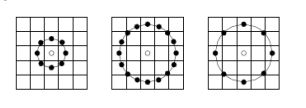
\includegraphics{lbpam.JPG}
	\caption[LBP étendue]{LBP étendue \textit{(source :\cite{TIM})}}
	\label{fig:lbpam}
\end{figure}

Dans la figure \ref{fig:lbpam} sont représentés les entourages $(8,1)$, $(16,2) $et $(8,2)$. Dans cette nouvelle représentation ne sont gardés que les patterns uniformes. Un pattern est dit uniforme s'il ne présentent pas plus de deux transitions '0-1' ou '1-0' et de manière circulaire. Ainsi 00110000 et
10000001 sont uniformes tandis que 10010001 et 10011101 ne le sont pas. Ojala et al. \cite{OJA} ont montré que les  LBPs  uniformes contiennent plus de 90\% de l'information d'une image. L'utilisation d'un code LBP uniforme, noté LBPu2 à deux avantages. Le premier est le  gain  en  mémoire  et  en  temps  calcul.  Le  deuxième  est  que  LBPu2 permet  de  détecter uniquement les textures locales importantes, comme les spots, les fins de ligne, les bords et les coins. Une propriété bien importante du code LBP est qu'il reste invariant aux changements uniformes globaux d'illumination, car le  LBP d'un pixel ne dépend que des différences entre son niveau de gris et celui de ses voisins.
\subsection{Processus de reconnaissance par LBP}
La reconnaissance de visage par LBP consiste en :
\begin{enumerate}
	\item calculer le LBP pour tous les pixels de l'image,
	\item l'image convertie est divisée en plusieurs sous-régions
pour lesquelles autant d'histogrammes LBP seront faits. Ainsi pour 4 sous-régions, 4
histogrammes seront générées. Ces derniers seront concaténés pour former une matrice à 2 dimensions appelée histogramme spatialement améliorée. Notons que les sous-régions peuvent se recouvrir et ne doivent pas nécessairement être rectangulaires.
	\item une métrique est utilisée pour la comparaison de deux histogrammes spatialement améliorées. Cette métrique doit établir une mesure de distance entre deux histogrammes simples et l'utilisation de poids pour rassembler les distances obtenues pour chaque sous région. La méthode 2 en 1 proposée par Ahonen et al. est la distance carrée de Chi balancée :
\begin{eqnarray}
\chi^2_w(x,\xi)=\sum_{j,i}{w_i\frac{(x_{i,j}-\xi_{i,j})^2}{x_{i,j}+\xi_{i,j}}}
\label{eq20}
\end{eqnarray}où x et $\xi$ sont des histogrammes spatialement améliorées normalisées à comparer, $i$ correspond à la $i$ ième valeur du $j$ ième sous-histogramme et $w_j$ est le poids accordé à la sous région $j$.
\end{enumerate}

Suite aux travaux de Ahonen et al., Tan et Triggs \cite{TAN}proposent trois nouveaux concepts qui permettent d'améliorer les performances de la méthodes LBP. Ces trois concepts sont les Local Trinary Patterns
(LTP), une méthode de prétraitement de l'image et enfin une méthode de mesure de
distance pour la comparaison d'échantillons au format LBP ou LTP.
\subsubsection*{Local Trinary Patterns}
Les Local Trinary Patterns sont une généralisation des  Local Binary Patterns au système ternaire. Ils ont été proposés  \cite{TAN} pour pallier aux problèmes de sensibilité qu'éprouve les LBP face aux bruits aléatoire et de quantification. 

Pour convertir en LTP, on attribue la valeur 0 aux pixels dont la valeur se trouve
dans un voisinage de la valeur du pixel central, 1 à ceux dont la valeur est au-delà de
ce voisinage et -1 à ceux dont la valeur est en dessous. La formulation mathématique
est la suivante pour un pixel périphérique $u$ d'un entourage à convertir, $i_c$ la valeur du pixel central et $t$ le voisinage : 
\[
s(u,i_c,t)=\left\{
\begin{array}{r c l}
1 &si& u\geq i_c + t\\
0 &si& \left|u-i_c\right|< t\\
-1 &si& u\geq i_c-t
\end{array}
\right.
\]
La figure \ref{fig:ltp} est une illustration de l'opérateur basique LTP.
\begin{figure}[htbp]
	\centering
		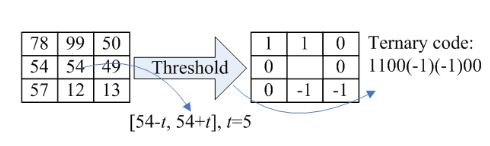
\includegraphics{ltp.JPG}
	\caption[illustration de l'opérateur basique LTP]{illustration de l'opérateur basique LTP (source : \cite{TAN})}
	\label{fig:ltp}
\end{figure}
Tan et Triggs ont par la suite divisé le code ternaire en deux codes binaires traités séparément et rassemblées ensuite lors de la phase de comparaison. Cette méthode à l'avantage de garder le système simple d'élimination
des patterns non-uniformes.
\begin{figure}[htbp]
	\centering
		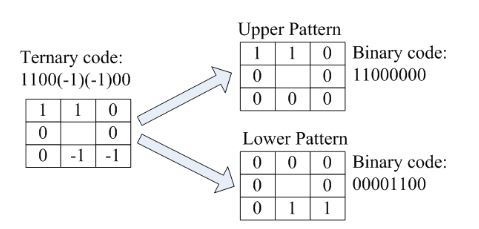
\includegraphics{tlpdivise.JPG}
	\caption{exemple de division d'un code TLP}
	\label{fig:tlp divise}
\end{figure}
\subsubsection*{Prétraitement de l'image}
La préparation de l'image s'effectue en trois étapes (cf.\cite{TAN}). 
\begin{enumerate}
	\item la correction Gamma
	\item le filtrage par différence de Gaussienne
	\item l'égalisation de contraste
\end{enumerate}
L'application de cette méthode de prétraitement à un même visage soumis à différentes conditions d'illumination
est illustrée à la figure 
\begin{figure}[htbp]
	\centering
		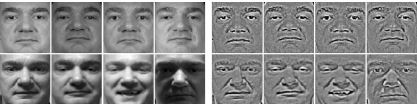
\includegraphics{pretraitement.JPG}
	\caption[Illustration du prétraitement de l'image de Tan et Triggs]{Illustration du prétraitement de l'image de Tan et Triggs (source : \cite{TAN})}
	\label{fig:pretraitement}
\end{figure}

\subsubsection*{Mesure de distance}
Tan et Triggs ont proposé une mesure de distance qui prend en compte l'organisation spatiale des LTP distribués sur l'entièreté de l'image. Les histogrammes ne sont plus utilisés. Pour comparer deux images X et Y, la méthode va regarder parmi les LTPs de même valeur de X celui qui est le plus proche et utiliser la distance qui les sépare pour incrémenter proportionnellement la distance globale. 

Autrement dit, pour un pattern de valeur k da Y, 
\begin{itemize}
	\item[\textbullet] on construit la matrice binaire $b^k_X$ qui représente la distribution des patterns k dans X.   
	\item[\textbullet] ensuite on construit les matrices $d^k_X$ de sorte qu'un élément $(i,j)$ de $d^k_X$ représente la distance entre $(i,j)$ et la position du plus proche pixel de X dont la valeur est k.
	\item[\textbullet] enfin, le calcul de la distance entre X et Y se fait par la formule
	\begin{eqnarray}
D(X,Y)=\sum_{pixels(i,j) de Y}{w(d_{X}^{k_Y(i,j)}{(i,j)})}
\label{eq20}
\end{eqnarray}
où w(d) est une fonction (à choisir) qui associe à une distance de pixel la pénalité correspondante. Tan et Triggs \cite{TAN} proposent la gaussienne $w(d)=exp^{(d/\sigma)^2/2)}$
et la troncation linéaire $w(d) = min(d; \tau)$ et disent que leurs performances sont similaires.
\end{itemize}

\section{Conclusion}
Dans ce chapitre, nous avons décrit deux méthodes de reconnaissance de visage : la méthode eigenface basée sur l'analyse en composante principale et la méthode LBP. Dans le chapitre suivant, nous mettrons ces deux algorithmes en œuvre et nous les testerons afin d'évaluer leurs performances.

\chapter{RÉSULTATS ET COMMENTAIRES}
\section{Introduction}
Dans ce chapitre, nous présentons les différents résultats obtenus après implémentation des algorithmes eigenfaces et Local Trinary Patterns. Pour cela, nous allons effectuer les tests sur les bases de données d'image ORL et YALE dans un premier temps, puis sur une base de donnée que nous allons créer.
\section{Bases de données de test}
\subsection{Base d'images ORL}\label{orl}
ORL est une base qui a été collectée entre avril 1992 et avril 1994 par le laboratoire AT\&T de
L'université  de Cambridge \footnote{http://web.mit.edu/emeyers/www/face\_databases.html\#orl consulté le 27/08/2016 à 22h36} . Elle est constituée de 40 personnes, chacune étant enregistrée sous 10 vues différentes. Les images sont de taille $112 \times 92$ pixels en format JPG et BMP
(portable  format  de  gris).  Pour  quelques  sujets,  les  images  ont  été  collectées  à  des  dates 
différentes,  avec  des  variations  dans  les  conditions  d'éclairage,  les  expressions  faciales 
(expression neutre, sourire et yeux fermés) et des occultations partielles par les lunettes. Toutes 
les  images  ont  été  collectées  sur  un  fond  foncé.  Les  poses  de  la  tête  présentent  quelques 
variations en profondeur par rapport à la pose frontale.

\begin{figure}[h]
 \caption[exemples d'images provenant de la base ORL]{exemples d'images provenant de la base ORL \\
source : http://web.mit.edu/emeyers/www/face\_databases.html\#orl}
	\centering
	
		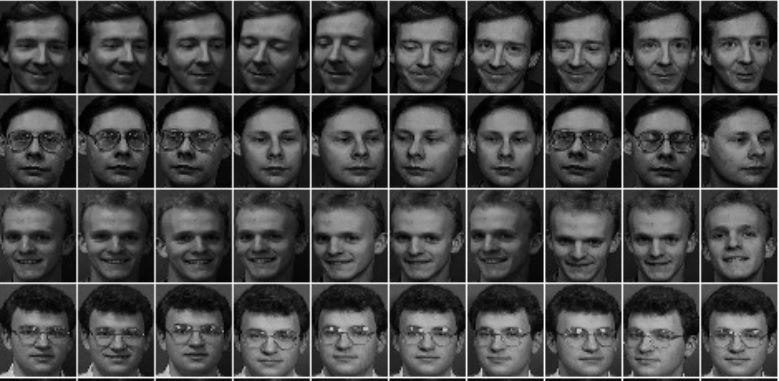
\includegraphics[width=450pt,height=250pt]{imagefromorl.JPG}
		
	\label{fig:imagefromorl}
\end{figure}
\newpage
\subsection{Base d'images YALE} \label{yale}

La base de données faciale Yale contient 165 images en niveaux de gris au format pgm de 15 personnes. Soit 11 images par sujet, les images ont chacune une expression du visage ou configuration différente : éclairage centrale, à gauche, à droite, port de verres ou non, heureux, triste, somnolent, surpris, et clin d'oeil.
\begin{figure}[htbp]
	\centering
		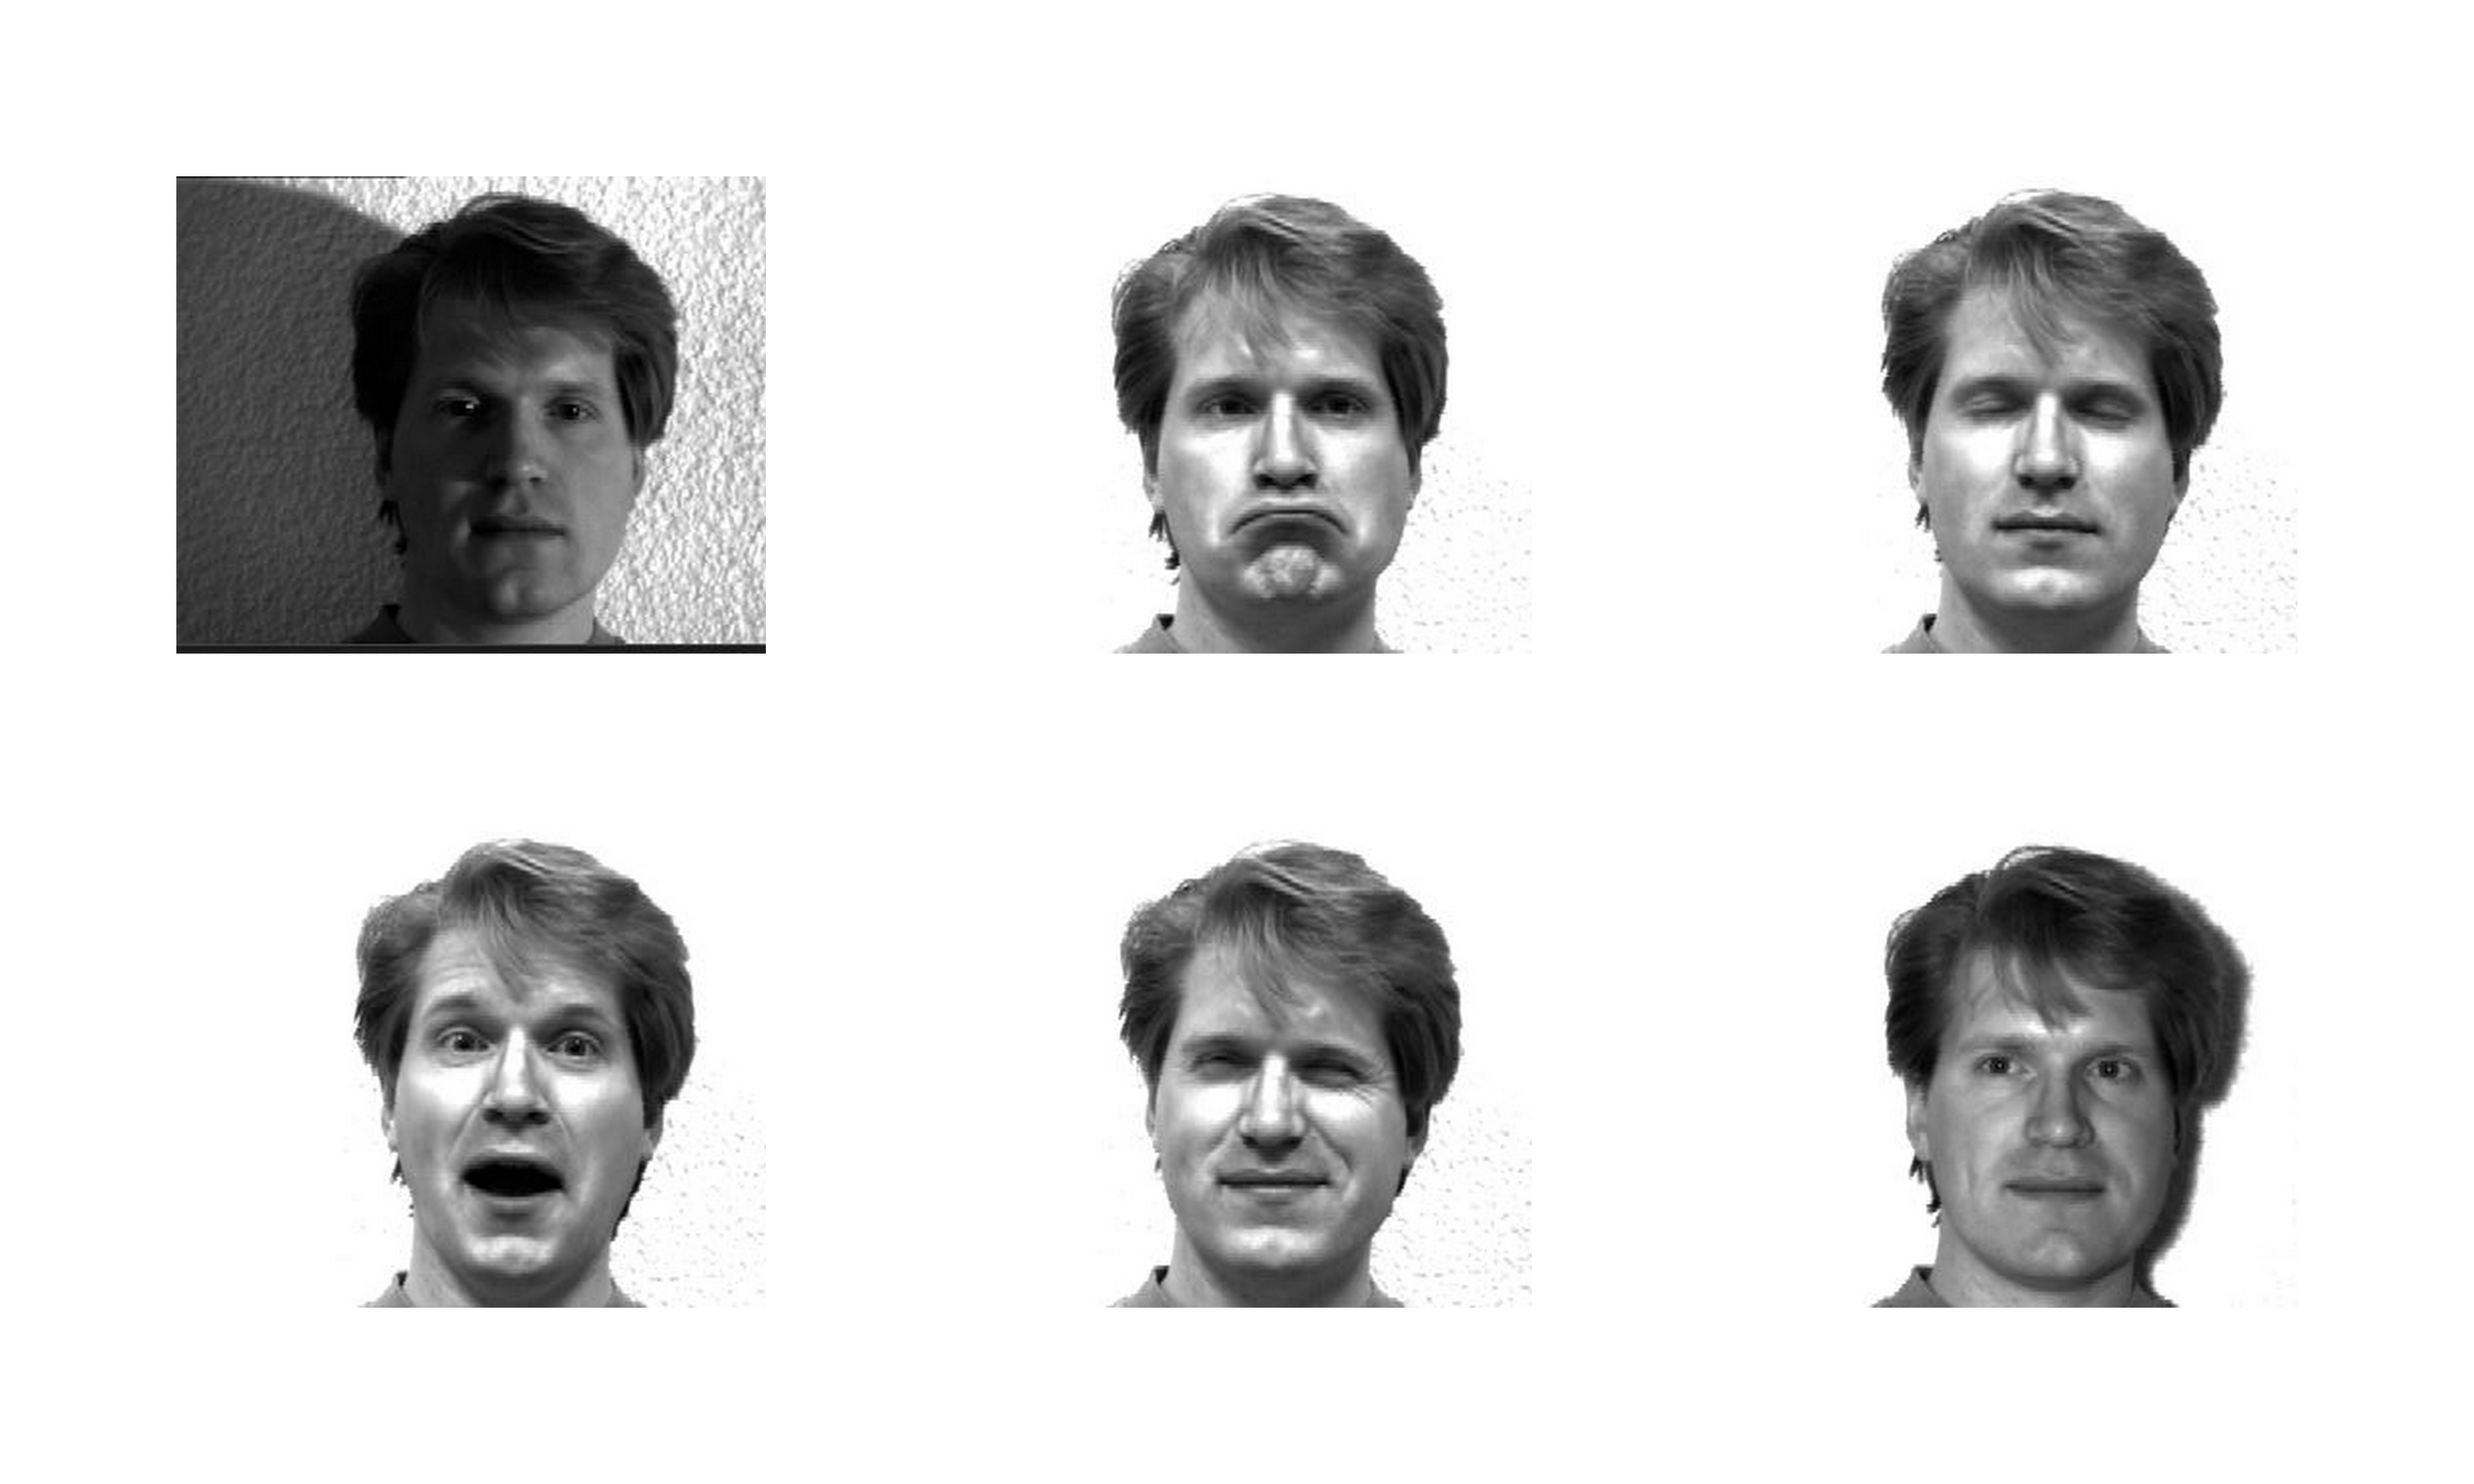
\includegraphics[width=450pt,height=200pt]{YAL.jpg}
		\caption[exemples d'images provenant de la base YALE ]{exemples d'images provenant de la base YALE \\
		source : http://web.mit.edu/emeyers/www/face\_databases.html\#yale}
	\label{fig:YAL}
\end{figure}

\subsection{Construire sa propre base de données d'images}
Pour construire une base de donnée d'images, on effectue des captures d'images de visage sur un ensemble d'individus. Ensuite on effectue un prétraitement (redimensionnement) sur l'ensemble des images capturées. Enfin les images sont groupées par dossiers en raison d'un individu par dossier.
\subsection{Séparation des bases de données}
Développer une application de reconnaissance faciale nécessite deux bases de données : une base de donnée d'apprentissage et une base de données pour les tests.
Dans les séries de test que nous avons effectué la base a été scindée de la façon suivante :
\begin{itemize}
	\item [\textbullet] Images apprentissages : Les 7 premières images servent pour la phase d'apprentissage.
	\item [\textbullet] Images Tests : Les 3 dernières images de chaque individu nous ont servies pour la réalisation des différents tests.
\end{itemize}
Le but est d'évaluer le taux de reconnaissance de  différents algorithmes présenté, en 
suivant un protocole de test basé sur la mesure de taux de reconnaissance. Le taux de reconnaissance est donné par l'expression 
$$taux\; de\; reconnaissance=\frac{nombre\; d'images\; de \;test\; reconnues}{nombre\; total\; d'images\; de \;test}$$
\section{Environnement de travail}

\subsection{Outils de développement}
Pour la réalisation de notre système de reconnaissance, nous avons utilisé le Java comme langage de programmation et la librairie OpenIMAJ. OpenIMAJ est un ensemble de librairies et d'outils pour l'analyse et la génération des contenus multimédia \footnote{http://www.openimaj.org}.  OpenIMAJ est principalement développé et maintenu par une équipe de chercheurs universitaires en électronique et d'informatique à l'Université de Southampton.
\nocite{OPEN}
\nocite{TUTO}
C'est possible d'écrire avec OpenIMAJ des programmes qui utilisent les bibliothèques dans toute langage JVM qui supporte
l'interopérabilité de Java, tel que Groovy, Jython, JRuby ou Scala. OpenIMAJ peut être exécuté même sur les téléphones Androïd et les tablettes.

OpenIMAJ est structurée en un grand nombre de librairies pouvant être utilisées de manière indépendantes. Les modules que nous avons utilisés sont : 
\begin{itemize}
	\item [\textbullet]  le module \textit{core} :  pour les modules qui contiennent les fonctionnalités usagée à travers les bibliothèques OpenIMAJ
	\item [\textbullet] le module \textit{core-image} : qui contient des définitions des images, les images élémentaires et les composants connectés.  Inclut le chargement, la sauvegarde et affichage des images.
	\item [\textbullet] le module \textit{core-vidéo} : qui contient des définitions d'un type de vidéo et fonctionnalités pour afficher et traiter des vidéos.
	\item [\textbullet]le module \textit{core-math} : mises en œuvre des outils mathématiques qui incluent géométrie, matrice et opérateurs statistiques.
		\item [\textbullet] le module \textit{image} : qui contient tout ce qui est relative aux images.
		\item [\textbullet] le module \textit{image-processing} : c'est une implémentation de nombreux algorithmes opérant sur les images comme la convolution, le redimensionnement, \ldots
		\item [\textbullet] le module \textit{image-local-features} :	qui contient des méthodes pour l'extraction de traits locaux
		\item [\textbullet] le module \textit{vidéo} : qui contient tout ce qui est relative aux flux vidéos.
		\item [\textbullet] le module \textit{vidéo-processing} : qui contient plusieurs fonctions de traitement de la vidéo.
		\item [\textbullet] le module \textit{machine-learning} : c'est un module dédiée à l'apprentissage automatique.
		\item [\textbullet] le module \textit{nearest-neighbour} : contient une implémentation de l'algorithme des K-plus proches voisins et autres méthodes d'approximation.
\end{itemize}
\section{Présentation de l'application}

Dans cette partie, nous présentons notre système de reconnaissance.
\subsection{Interface d'accueil}
C'est l'interface de communication entre les utilisateurs et le système de reconnaissance. Elle est assez intuitive et présente les différentes fonctionnalités du système (identification de visage, visage propre, suivi d'un visage, \ldots)
\begin{figure}[htbp]
	\centering
		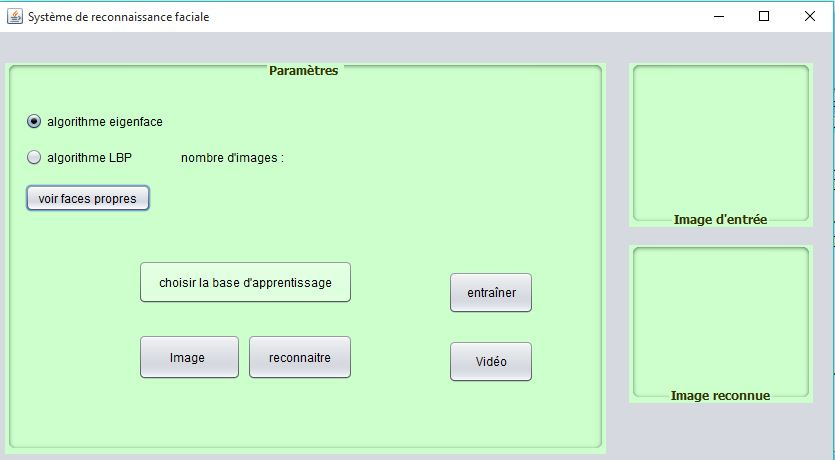
\includegraphics[width=450pt,height=350pt]{accueil.JPG}
	\caption{interface d'accueil du système de reconnaissance}
	\label{fig:accueil}
\end{figure}
\begin{itemize}
	\item [\textbullet]les boutons radio '\textit{algorithme eigenface}' et '\textit{algorithme LBP}' permettent de sélectionner l'algorithme de reconnaissance à utiliser.
	\item [\textbullet] Si l'algorithme eigenface est sélectionné, alors le bouton '\textit{voir faces propres}' apparaît. Ce dernier permet de voir les faces propres construites par la technique ACP.
	\item [\textbullet] le bouton '\textit{choisir la base d’apprentissage}' permet de charger la base de données d'images à utiliser.
	\item [\textbullet] une fois la base choisie, le bouton '\textit{entraîner}' permet d'entraîner l'algorithme de reconnaissance sur cette base.
	\item [\textbullet] le bouton '\textit{image}' permet de charger l'image d'entrée du système de reconnaissance. une fois l'image choisie, elle apparaît dans le panneau latéral droit à l'emplacement '\textit{image d'entrée}'
	\item [\textbullet] le bouton '\textit{reconnaître}' permet de lancer la reconnaissance.
	
	\item [\textbullet] le bouton '\textit{vidéo}' permet de lancer une reconnaissance en prenant comme entrée la vidéo capturée directement depuis un périphérique.
	\end{itemize}
	
	\subsection{Test de l'algorithme eigenface}
	
	\subsubsection{Sur la base de donnée ORL}
	\begin{enumerate}
		\item \textbf{Choix de la base d'apprentissage}
		
		\begin{figure}[htbp]
			\centering
				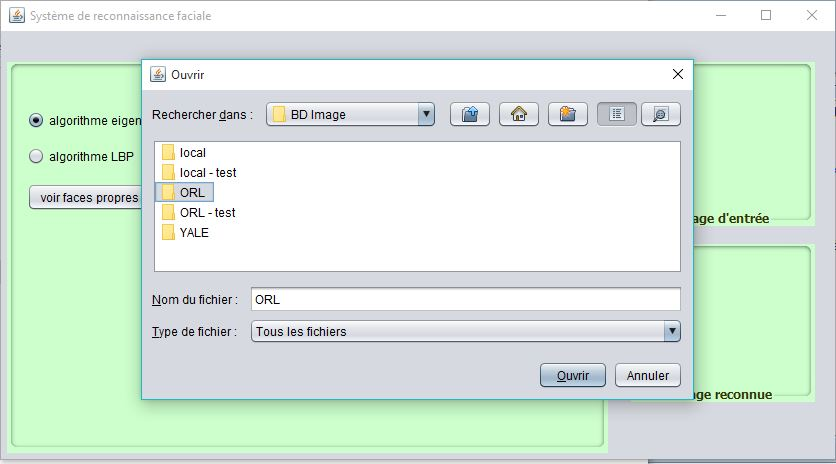
\includegraphics[width=450pt,height=350pt]{choixORL.JPG}
			\caption{choix de la base d'image ORL}
			\label{fig:choixORL}
		\end{figure}
		\newpage
			\item \textbf{entraînement de l'algorithme sur la base d'image}
			
			On sélectionne dans l'arborescence des fichiers le répertoire contenant la base de données ORL. Puis on clique sur le bouton '\textit{entraîner}'.
			\begin{figure}
				\centering
					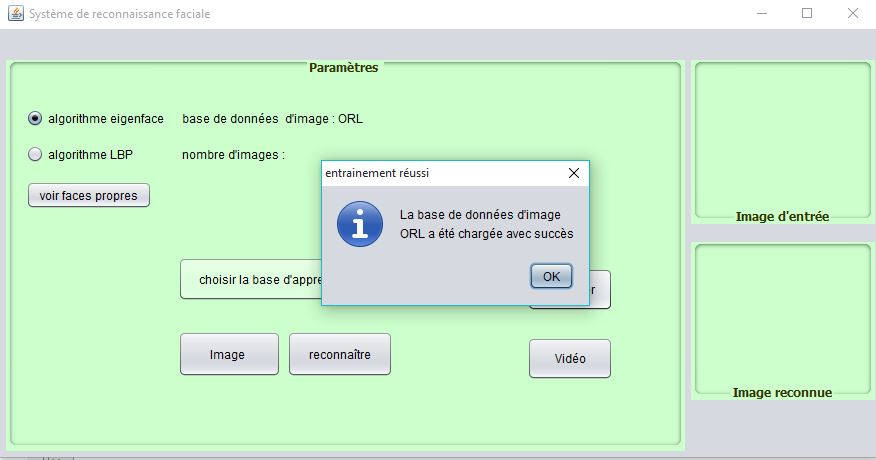
\includegraphics[width=450pt,height=350pt]{dbcharged.JPG}
				\caption{apprentissage de l'algorithme}
				\label{fig:dbcharged}
			\end{figure}
			\newpage
				\item \textbf{voir les faces propres.}
				
			Pour visualiser quelques faces propres de la base d'images, on sélectionne le bouton '\textit{voir faces propres}'
			
			\begin{figure}[htbp]
				\centering
					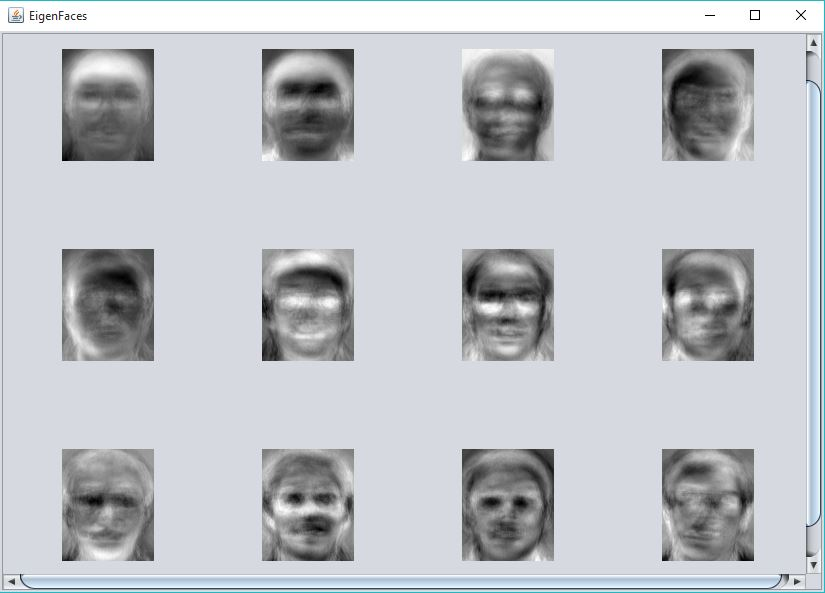
\includegraphics[width=450pt,height=350pt]{eigenORL.JPG}
				\caption{quelques faces propres de la base ORL}
				\label{fig:eigenORL}
			\end{figure}
			\newpage
			\item \textbf{identifier un visage.}
			
			Pour cela, cliquer sur le bouton '\textit{image}' et choisir l'image d'entrée. L'image d'entrée doit être de même taille que celles de la base d'apprentissage pour ce cas. 
			
			
			\begin{figure}[htbp]
				\centering
					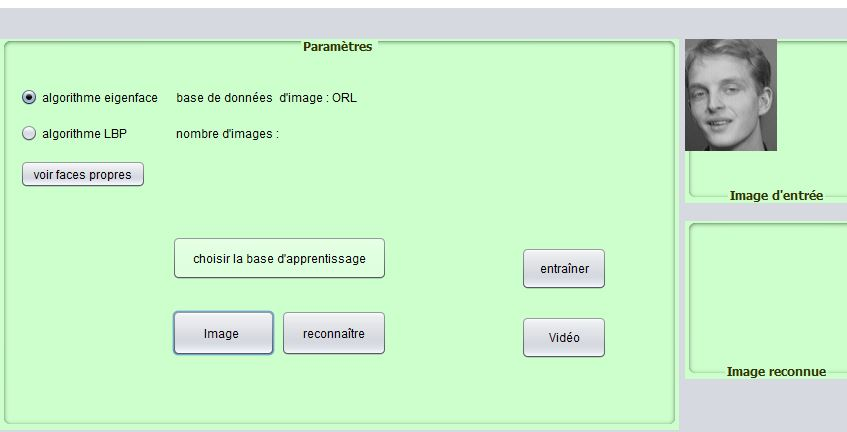
\includegraphics[width=450pt,height=220pt]{imageorlcharge.JPG}
				\caption{chargement d'une image de test}
				\label{fig:imageorlcharge}
			\end{figure}
		
	Puis on lance la reconnaissance en cliquant sur le bouton reconnaître.
			\begin{figure}[htbp]
				\centering
					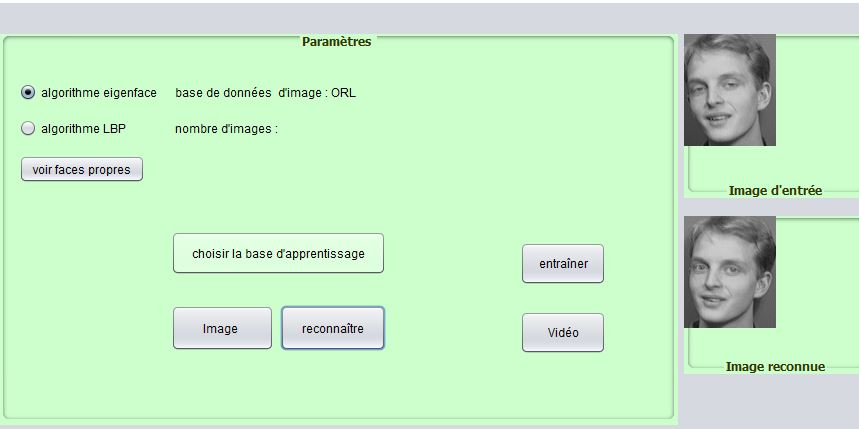
\includegraphics[width=450pt,height=220pt]{imageorlRecognize.JPG}
				\caption{visage reconnue}
				\label{fig:imageorlcharge}
			\end{figure}
		\end{enumerate}	
		
		 \subsubsection{Sur la base de donnée YALE}
		
		Le processus est le même que pour la base de donnée ORL, sauf que les images utilisés pour l'entraînement et le test proviennent de la base YALE. Un exemple de reconnaissance est représenté à la figure \ref{fig:eigenYale} .
		
		\begin{figure}[htbp]
			\centering
				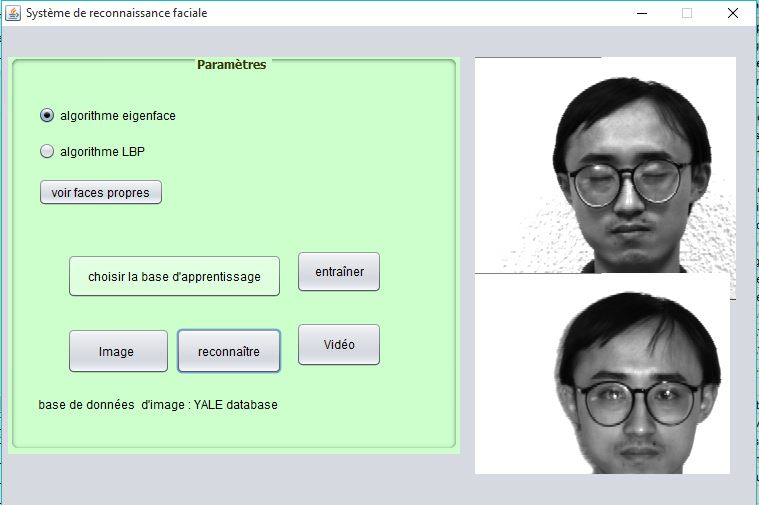
\includegraphics[width=400pt,height=200pt]{eigenYale.JPG}
			\caption{exemple de reconnaissance sur la base de données YALE}
			\label{fig:eigenYale}
		\end{figure}
			\subsection{Identifier un visage à partir d'un flux vidéo.}
			
			Pour cela, on choisit une base de donnée image potentielle. Dans ce cas, ça sera la base de donnée 'locale', puis on lance la reconnaissance en cliquant sur le bouton '\textit{video}'. La figure ci-dessous représente quelques images prélevées dans cette base.
			
			\begin{figure}[htbp]
				\centering
					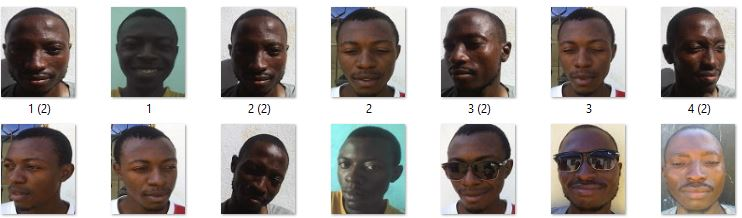
\includegraphics[width=450pt,height=170pt]{bdlocal.JPG}
				\caption{quelques images de la base de données 'local'}
				\label{fig:bdlocal}
			\end{figure}
					
			\begin{figure}[htbp]
				\centering
					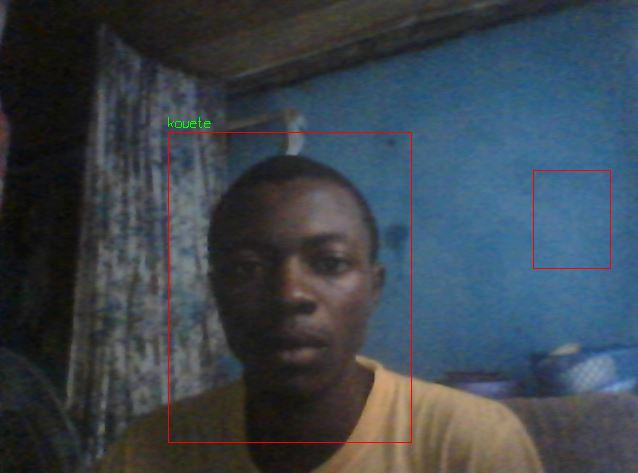
\includegraphics[width=350pt,height=200pt]{reconVideo.JPG}
				\caption{reconnaissance à partir d'un flux vidéo}
				\label{fig:reconVideo}
			\end{figure}
			
\newpage
	\subsubsection{Commentaires}
	Le taux de reconnaissance de l'algorithme eigenface sur la base de données ORL est de 93,20\% en moyenne pour une base d'entraînement de 6*40=240 images et une base de 4*40=160 pour les tests. Le temps d'apprentissage mesuré est d'environ 16 secondes contre un temps de reconnaissance d'environ une seconde. 
	
	Le même algorithme appliqué sur la base YALE séparée en une base de 6*15=90 images pour l'entraînement et une base de 5*15=75 images pour les tests donne un taux de reconnaissance de 78.67\% en moyenne.  Le temps d'apprentissage mesuré est d'environ 24 secondes contre un temps de reconnaissance de 14 secondes. 
	
		\subsection{Test de l'algorithme LBP}
Les tests se déroulent de la même manière que pour l'algorithme eigenface. Il suffit d'activer le bouton radio 'algorithme LBP' pour choisir d'utiliser l'algorithme LBP. Des exemples de test sont illustrés par les figures \ref{fig:reconLBP1} et \ref{fig:reconLBP2} ci-dessous.		
		\begin{figure}[htbp]
			\centering
				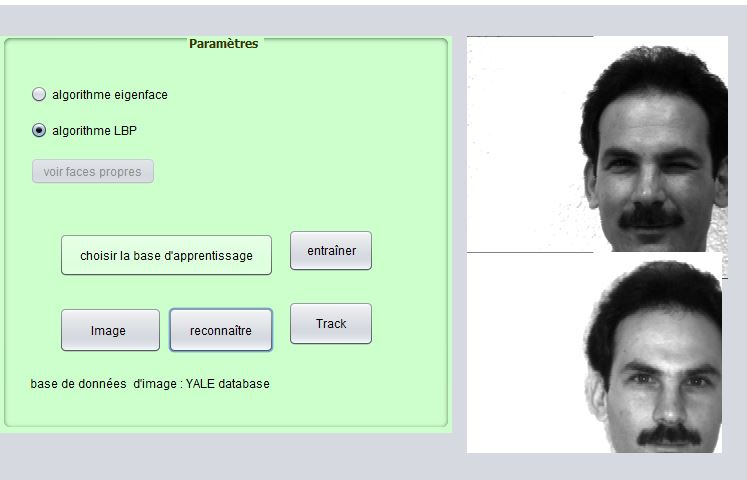
\includegraphics[width=350pt,height=200pt]{reconLBP1.JPG}
			\caption{algorithme LBP appliqué sur la base YALE}
			\label{fig:reconLBP1}
		\end{figure}	
		
		\begin{figure}[htbp]
			\centering
				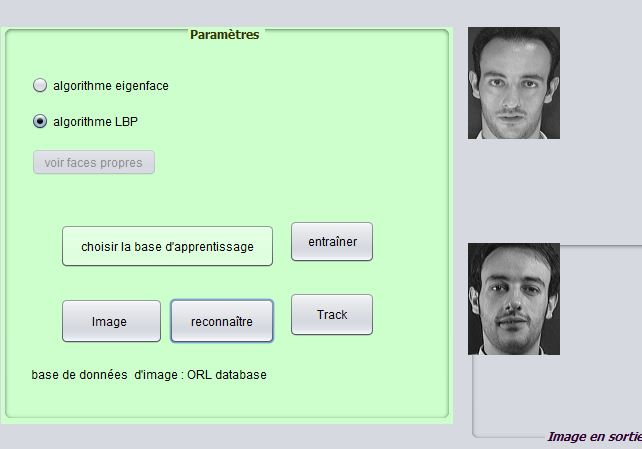
\includegraphics[width=350pt,height=250pt]{reconLBP2.JPG}
			\caption{algorithme LBP appliqué à la base ORL}
			\label{fig:reconLBP2}
		\end{figure}
		\newpage
	L'un des points forts de l'algorithme LBP est sa capacité à pouvoir opérer sur des bases d'images constituées d'un seul échantillon. Cet avantage peut être utilisé pour pister un individu par un réseau de caméra. Une application est illustrée par les captures suivantes :
	
	\begin{enumerate}
		\item Dans un premier temps, le système détecte le visage. Ce dernier peut alors être enregistré en faisant une combinaison des touches Ctrl et S.
		\begin{figure}[htbp]
		\centering
			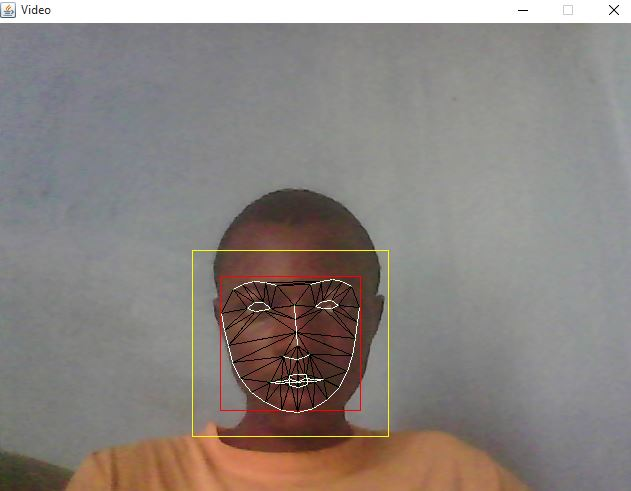
\includegraphics[width=350pt,height=200pt]{track1.JPG}
		\caption{détection et capture du visage}
		\label{fig:track 1}
	\end{figure}
	\item L'utilisateur entre une information caractérisant le visage capturée, puis valide. Le système s'entraîne alors à reconnaître le visage enregistré. Par exemple un nom.
	\begin{figure}[htbp]
		\centering
			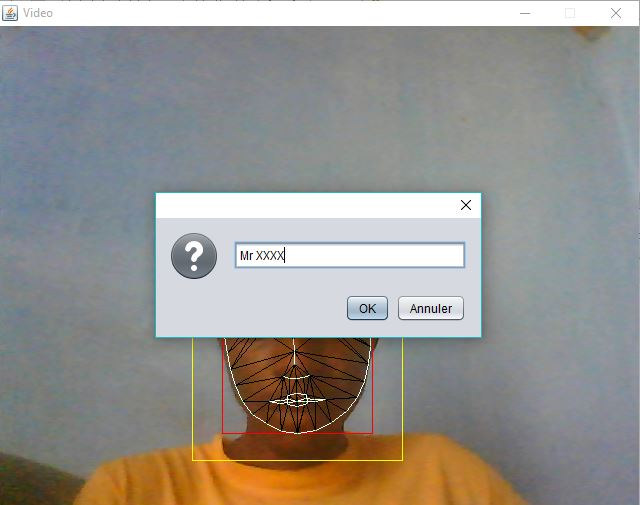
\includegraphics[width=350pt,height=200pt]{track2.JPG}
		\caption{enregistrement du visage}
		\label{fig:track 1}
	\end{figure}
	
	\item Le visage est alors reconnu à chaque fois qu'il passe dans le champ de vision du périphérique de capture.
	
	\begin{figure}[htbp]
		\centering
			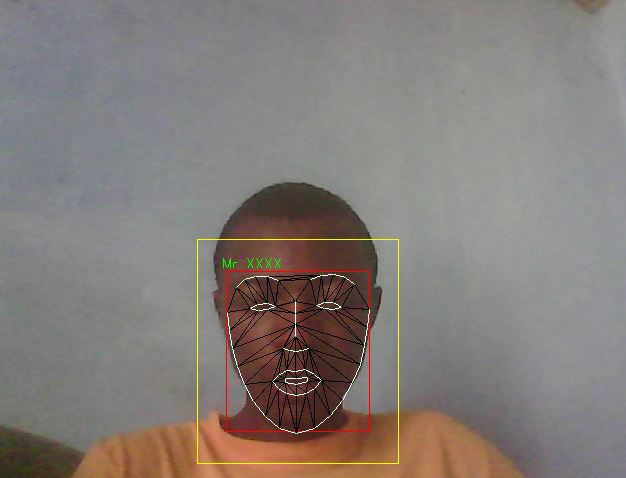
\includegraphics[width=350pt,height=200pt]{track3.JPG}
		\caption{suivi du visage}
		\label{fig:track 1}
	\end{figure}
	\end{enumerate}
	
	
	
		\subsubsection{Commentaires}
	Le taux de reconnaissance de l'algorithme LBP sur la base de données ORL est de 96.6\% pour les mêmes bases d'apprentissage et de test que précédemment. Le temps d'apprentissage mesuré est d'environ 22 secondes contre un temps de reconnaissance d'environ 13 secondes. 
	
	Le même algorithme appliqué sur la base YALE séparée en une base de 7*15=105 images pour l'entraînement et une base de 4*15=760 images pour les tests donne un taux de reconnaissance de 46.67\% seulement. Ceci est du au fait que les images de la base YALE présentent de variations extérieures. Le temps d'apprentissage mesuré est d'environ 16 secondes contre un temps de reconnaissance de 8 secondes. 
	\subsection{Comparaison des performances}
	Le tableau ci-dessous est une comparaison des performances des algorithmes eigenface et LBP sur les bases de données ORL et YALE.
	
	\begin{table}[htbp]
		\centering
			\begin{tabular}{|l|c|c |}
				\hline &algorithme eigenface& algorithme LBP\\
				\hline ORL  & 93.2\%& 96.6\%\\
				\hline YALE & 78.67\%& 46.67\%\\
				\hline
			\end{tabular}
		\caption{performance des algorithmes LBP et eigenface sur les bases d'images ORL et YALE}
		\label{tab:performanceDesAlgorithmesLBPEtEigenfaceSurLesBasesDImagesORLEtYALE}
	\end{table}
\section{Conclusion}
Nous avons présenté dans ce chapitre les différents résultats obtenus après implémentation et tests des algorithmes LBP et eigenfaces. Les bases de données d'images sont ORL( section \ref{orl}), YALE (\ref{yale}) et une base nommée 'local' que nous avons nous même créée. Il est à noter que le temps d'exécution des algorithmes croît avec le nombre d'image contenue dans la base de données. Par ailleurs l'algorithme LBP s'avère un peu plus rapide et est mieux adapté pour le problème à un échantillon.
\nocite{TRACK}

\chapter*{CONCLUSION ET PERSPECTIVES}\addcontentsline{toc}{chapter}{CONCLUSION ET PERSPECTIVES}

Dans ce travail, nous nous sommes intéressé au problème de reconnaissance faciale. Nous avons mis sur pied un système de reconnaissance faciale basé sur les algorithmes Eigenface et LBP qui représentent deux des algorithmes de reconnaissance les plus utilisés. La méthode de détection de visage utilisé dans les deux cas est l'algorithme de Viola et Jones \cite{VIO}. C'est une méthode largement reconnue comme fonctionnant en temps réel et avec de très bon résultats ( plus de 98\% pour des visages présentés de face, plus de 94\% pour des visages faisant moins de 20\degres. Nous avons trouver ces résultats assez convaincant pour l'utilisation de l'algorithme de Viola et Jones dans notre application.

 L'algorithme Eigenface est basé sur la technique mathématique ACP (Analyse en composantes principales) qui est un moyen de simplifier en ensemble de données en réduisant sa dimension. Elle  est  utilisée  pour  représenter efficacement les images  de visages, qui peuvent être approximativement  reconstruites à partir d'un petit ensemble de poids et d'une image de visage standard. L'algorithme LBP quant à elle consiste à construire l'histogramme d'une image en utilisant le code LBP de tous ces pixels préalablement calculé. L'histogramme LBP permet de construire un vecteur de  caractéristiques représentant l'image faciale.

Les systèmes de reconnaissance sont pour la plupart influencés par les problèmes d'illumination, de variations de pose et d'éclairage. Nous avons proposé dans ce mémoire quelques solutions à ce problème. Mais malgré les progrès réalisés, les variations de pose restent un sérieux défis à relever dans la reconnaissance dans des environnements extérieurs, dont suscite des efforts de la part des chercheurs. Néanmoins l'ACP est une approche efficace et simple pour remédier à ce problème.

En guise de perspectives, ce travail peut être étendu dans un premier temps par l'amélioration de ses capacités à résister aux variations d'environnements. Et dans un second temps par 
la conception et la mise en œuvre d'un système de reconnaissance à performances assez hautes (utilisant par exemple la reconnaissance en 3D), pouvant servir à pister un individu à l'aide d'un réseau de caméras. 

\addcontentsline{toc}{chapter}{Bibliographie}
\bibliographystyle{plain} % or try unsrtnat or plainnat 
\bibliography{biblio} % refers to biblio.bib

%%%%%%%%%%%%%%%%%%%%%%%%%%%%%%%%%%%%%%%%%%%%%%%%%%%%%%%%%%%%%
%% APPENDICES
%%%%%%%%%%%%%%%%%%%%%%%%%%%%%%%%%%%%%%%%%%%%%%%%%%%%%%%%%%%%%
\appendix
%% ==> Write your text here or include other files.

%\input{FileName} %You need a file 'FileName.tex' for this.


\end{document}

